%----------
%   WARNING
%----------

% This Guide contains Library recommendations based mainly on APA and IEEE styles, but you must always follow the guidelines of your TFG Tutor and the TFG regulations for your degree.

% THIS TEMPLATE IS BASED ON THE APA STYLE


%----------
% DOCUMENT SETTINGS
%----------

\documentclass[12pt]{report} % font: 12pt

% margins: 2.5 cm top and bottom; 3 cm left and right
\usepackage[
a4paper,
vmargin=2.5cm,
hmargin=3cm
]{geometry}

% Paragraph Spacing and Line Spacing: Narrow (6 pt / 1.15 spacing) or Moderate (6 pt / 1.5 spacing)
\renewcommand{\baselinestretch}{1.15}
\parskip=6pt

% Color settings for cover and code listings
\usepackage[table]{xcolor}
\definecolor{azulUC3M}{RGB}{0,0,102}
\definecolor{gray97}{gray}{.97}
\definecolor{gray75}{gray}{.75}
\definecolor{gray45}{gray}{.45}

% PDF/A -- Important for its inclusion in e-Archive. PDF/A is the optimal format for preservation and for the generation of metadata: http://uc3m.libguides.com/ld.php?content_id=31389625.

% In the template we include the file OUTPUT.XMPDATA. You can download that file and include the metadata that will be incorporated into the PDF file when you compile the memoria.tex file. Then upload it back to your project.
\usepackage[a-1b]{pdfx}

% LINKS
\usepackage{hyperref}
\hypersetup{colorlinks=true,
	linkcolor=black, % links to parts of the document (e.g. index) in black
	citecolor=black, % citations in black
	urlcolor=blue} % links to resources outside the document in blue

% MATH EXPRESSIONS
\usepackage{amsmath,amssymb,amsfonts,amsthm}

% Character encoding
\usepackage{txfonts}
\usepackage[T1]{fontenc}
\usepackage[utf8]{inputenc}

% English settings
\usepackage[english]{babel}
\usepackage[babel, english=american]{csquotes}
\AtBeginEnvironment{quote}{\small}

% Footer settings
\usepackage{fancyhdr}
\pagestyle{fancy}
\fancyhf{}
\renewcommand{\headrulewidth}{0pt}
\rfoot{\thepage}
\fancypagestyle{plain}{\pagestyle{fancy}}

% DESIGN OF THE TITLES of the parts of the work (chapters and epigraphs or sub-chapters)
\usepackage{titlesec}
\usepackage{titletoc}
\titleformat{\chapter}[block]
{\large\bfseries\filcenter}
{\thechapter.}
{5pt}
{\MakeUppercase}
{}
\titlespacing{\chapter}{0pt}{0pt}{*3}
\titlecontents{chapter}
[0pt]
{}
{\contentsmargin{0pt}\thecontentslabel.\enspace\uppercase}
{\contentsmargin{0pt}\uppercase}
{\titlerule*[.7pc]{.}\contentspage}

\titleformat{\section}
{\bfseries}
{\thesection.}
{5pt}
{}
\titlecontents{section}
[5pt]
{}
{\contentsmargin{0pt}\thecontentslabel.\enspace}
{\contentsmargin{0pt}}
{\titlerule*[.7pc]{.}\contentspage}

\titleformat{\subsection}
{\normalsize\bfseries}
{\thesubsection.}
{5pt}
{}
\titlecontents{subsection}
[10pt]
{}
{\contentsmargin{0pt}
	\thecontentslabel.\enspace}
{\contentsmargin{0pt}}
{\titlerule*[.7pc]{.}\contentspage}


% Tables and figures settings
\usepackage{multirow} % combine cells
\usepackage{booktabs} % horizontal rules in tables
\usepackage{microtype} % keeps long lines inside the margins
\usepackage{caption} % customize the title of tables and figures
\usepackage{floatrow} % we use this package and its \ ttabbox and \ ffigbox macros to align the table and figure names according to the defined style.
\usepackage{array} % with this package we can define in the following line a new type of column for tables: custom width and centered content
\newcolumntype{P}[1]{>{\centering\arraybackslash}p{#1}}
\DeclareCaptionFormat{upper}{#1#2\uppercase{#3}\par}
\usepackage{graphicx}
\graphicspath{{imagenes/}} % images folder

% Table layout for social sciences and humanities
\captionsetup*[table]{
	justification=raggedright,
	labelsep=newline,
	labelfont=small,
	singlelinecheck=false,
	labelfont=bf,
	font=small,
	textfont=it
}

% Figure layout for social sciences and humanities
\captionsetup[figure]{
	%name=Figura,
	singlelinecheck=off,
	labelsep=newline,
	font=small,
	labelfont=bf,
	textfont=it
}
\floatsetup[figure]{
    style=plaintop,
    heightadjust=caption,
    footposition=bottom,
    font=small
}

% Figures and tables footnote layout
\captionsetup*[floatfoot]{
    footfont={small, up}
}

% FOOTNOTES
\usepackage{chngcntr} % continuous numbering of footnotes
\counterwithout{footnote}{chapter}

% CODE LISTINGS
% support and styling for listings. More information in  https://es.wikibooks.org/wiki/Manual_de_LaTeX/Listados_de_código/Listados_con_listings
\usepackage{listings}

% Custom listing
\lstdefinestyle{estilo}{ frame=Ltb,
	framerule=0pt,
	aboveskip=0.5cm,
	framextopmargin=3pt,
	framexbottommargin=3pt,
	framexleftmargin=0.4cm,
	framesep=0pt,
	rulesep=.4pt,
	backgroundcolor=\color{gray97},
	rulesepcolor=\color{black},
	%
	basicstyle=\ttfamily\footnotesize,
	keywordstyle=\bfseries,
	stringstyle=\ttfamily,
	showstringspaces = false,
	commentstyle=\color{gray45},
	%
	numbers=left,
	numbersep=15pt,
	numberstyle=\tiny,
	numberfirstline = false,
	breaklines=true,
	xleftmargin=\parindent
}

\captionsetup*[lstlisting]{font=small, labelsep=period}

\lstset{style=estilo}
\renewcommand{\lstlistingname}{\uppercase{Code}}


% REFERENCES

% APA bibliography setup
\usepackage[style=apa, backend=biber, natbib=true, hyperref=true, uniquelist=false, sortcites]{biblatex}

\addbibresource{referencias.bib} % The references.bib file in which the bibliography used should be


%-------------
%	DOCUMENT
%-------------

\begin{document}
\pagenumbering{roman} % Roman numerals are used in the numbering of the pages preceding the body of the work.

%----------
%	COVER
%----------
\begin{titlepage}
	\begin{sffamily}
	\color{azulUC3M}
	\begin{center}
		\begin{figure}[H] % UC3M Logo
			\makebox[\textwidth][c]{
\includegraphics[width=16cm]{logo_UC3M.png}}
		\end{figure}
		\vspace{2.5cm}
		\begin{Large}
			Master Degree in Statistics for Data Science\\
			 2025-2026\\ % Academic year
			\vspace{2cm}
			\textsl{Master Thesis}
			\bigskip

		\end{Large}
		 	{\Huge ``Comparing Smoothing Procedures for Conditional Density Estimation in Factor-Augmented Quantile Regressions''}\\
		 	\vspace*{0.5cm}
	 		\rule{10.5cm}{0.1mm}\\
			\vspace*{0.9cm}
			{\LARGE Marel Arturo Castro}\\
			\vspace*{1cm}
		\begin{Large}
			Esther Ruiz Ortega Ph.D.\\
			Madrid, Spain, September 2026\\
		\end{Large}
	\end{center}
	\vfill
	\color{black}
	\fbox{
	\begin{minipage}{\linewidth}
    	\textbf{AVOID PLAGIARISM}\\
    	\footnotesize{The University uses the \textbf{Turnitin Feedback Studio} for the delivery of student work. This program compares the originality of the work delivered by each student with millions of electronic resources and detects those parts of the text that are copied and pasted. Plagiarizing in a TFM is considered a  \textbf{\underline{Serious Misconduct}}, and may result in permanent expulsion from the University.}\end{minipage}}

	% IF OUR WORK IS TO BE PUBLISHED UNDER A CREATIVE COMMONS LICENSE, INCLUDE THESE LINES. IS THE RECOMMENDED OPTION.
	\noindent
\includegraphics[width=4.2cm]{creativecommons.png}\\ % Creative Commons Logo
    \footnotesize{This work is licensed under Creative Commons \textbf{Attribution – Non Commercial – Non Derivatives}}

	\end{sffamily}
\end{titlepage}

\newpage % blank page
\thispagestyle{empty}
\mbox{}

%----------
%	ABSTRACT AND KEYWORDS
%----------
\renewcommand\abstractname{\large\bfseries\filcenter\uppercase{Summary}}
\begin{abstract}
\thispagestyle{plain}
\setcounter{page}{3}

	% Write your abstract
	This thesis compares two procedures for converting the conditional quantiles of a factor-augmented quantile regression into a full conditional density: the parametric skew-$t$ fit of \textcite{adrian2019vulnerable} and the piecewise-linear procedure of \textcite{mitchell2024constructing}. In a Monte Carlo study with Gaussian, skew-$t$, and bimodal data-generating processes, the piecewise-linear smoother reduces the mean integrated squared error by roughly 38 percent when the true density is bimodal, while the skew-$t$ is more accurate on MISE under the Gaussian benchmark. In an application to one-quarter-ahead US GDP growth with factors extracted from the FRED-QD database, the two smoothers give similar densities in 2006 Q2 and differ most clearly in 2008 Q4, where the piecewise-linear density is multimodal. The skew-$t$ fit reaches a parameter bound at 47 percent of the dates in-sample and 50 percent out-of-sample. In an out-of-sample evaluation over 143 quarters, neither smoother is significantly more accurate on any variant of the continuous ranked probability score.

	\textbf{Keywords:} Conditional density estimation, Quantile regression, Factor models, Skew-$t$ distribution, Density forecast evaluation, Growth-at-Risk

	\vfill
\end{abstract}
	\newpage % Blank page
	\thispagestyle{empty}
	\mbox{}


%----------
%	Dedication
%----------

\chapter*{Dedication}

\setcounter{page}{5}

\vspace*{\fill}

\begin{center}
Dedicated to

\vspace{1cm}

Alexis Octavio Guerrero, \\
Kelvin Antonio Rubio, \\
Luis Alexander Gonzalez, \\
Miguel Eliseo Carrion, \\
and to my beloved Ning Tian.
\end{center}

\vspace*{\fill}

\newpage % blank page
\thispagestyle{empty}
\mbox{}


%----------
%	TOC
%----------

%--
% TOC
%-
\tableofcontents
\thispagestyle{fancy}

\newpage % blank page
\thispagestyle{empty}
\mbox{}

%--
% List of figures. If they are not included, comment the following lines
%-
\listoffigures
\thispagestyle{fancy}

\newpage % blank page
\thispagestyle{empty}
\mbox{}

%--
% List of tables. If they are not included, comment the following lines
%-
\listoftables
\thispagestyle{fancy}

\newpage % blankpage
\thispagestyle{empty}
\mbox{}


%----------
%	THESIS
%----------
\clearpage
\pagenumbering{arabic} % numbering with Arabic numerals for the rest of the document.

% IMPORTANT: Latex special characters are: # $ % & \ ^ _ { } ~. To avoid mistakes when compiling try writing \ before. For: \ use \textbackslash ; for ^ \textasciicircum and ~ \textasciitilde.

%----------
%	1. INTRODUCTION
%----------

\chapter{Introduction}
\label{ch:intro}

Economic forecasts have traditionally focused on point predictions, such as expected GDP growth. A single point prediction, however, does not describe the uncertainty around that prediction or distinguish between a stable outcome and a substantial downside risk. This makes the full range of possible outcomes relevant for policy. The thesis builds on the framework of \textcite{adrian2019vulnerable}, henceforth ABG. The method first estimates conditional quantiles and then fits a four-parameter skew-$t$ distribution to those quantiles. ABG show that downside risk in US GDP growth varies substantially with financial conditions, while the upper part of the distribution is comparatively stable. Subsequent work has extended the quantile-regression stage by incorporating information from large macroeconomic datasets. Factor-augmented quantile regression (FA-QR) instead uses principal components to summarize information from a large panel of macroeconomic and financial variables before estimating the conditional quantiles.

The quantile-regression stage has received considerably more attention than the second-stage procedure used to convert the estimated quantiles into a density. The ABG skew-$t$ specification is unimodal by construction. If the conditional distribution is multimodal, the skew-$t$ specification cannot represent the separate modes and instead imposes a single unimodal density. \textcite{mitchell2024constructing}, henceforth MPZ, use a flexible piecewise-linear smoother and find evidence of multimodality in US GDP growth during crisis periods that the skew-$t$ specification does not capture.

This thesis examines how the choice of smoothing procedure affects the estimated conditional density and its out-of-sample forecast accuracy. To do so, we build a standard FA-QR pipeline using data from the FRED-QD database and compare these smoothers. We compare the ABG and piecewise-linear approaches first in a Monte Carlo simulation spanning symmetric, skewed, and bimodal shapes, and then in a real-world forecasting application for US GDP growth. The results show that the choice of smoother affects the estimated density, with the differences being most pronounced during periods of economic stress. Chapter~\ref{ch:faqr} describes the methodology, Chapter~\ref{ch:mc} presents the Monte Carlo study, Chapter~\ref{ch:empirical} presents the empirical application, and Chapter~\ref{ch:conclusion} concludes.

%----------
%	2. FA-QR
%----------

\chapter{Factor-Augmented Quantile Regression (FA-QR)}
\label{ch:faqr}

The FA-QR framework used in this thesis first extracts a small number of latent factors from a large panel of macroeconomic and financial series. Quantile regressions are then estimated using these factors, producing forecasts at a chosen grid of quantile levels. Finally, the estimated quantiles are smoothed into a full conditional density. The factor extraction and quantile regression steps are common across the smoothing procedures compared in this thesis and are set out in Sections~\ref{sec:factors} and~\ref{sec:qr}. The competing smoothing procedures are described in Section~\ref{sec:smoothing}, which sets out the parametric skew-$t$ procedure of ABG, the semi-parametric piecewise-linear procedure of Mitchell, Poon, and Zhu, and two further procedures that place the comparison in context. Section~\ref{sec:evaluation} sets out the metrics used to evaluate the resulting density forecasts.

\section{Factor extraction via principal components}
\label{sec:factors}

Let $X_t = (x_{1t}, \ldots, x_{Nt})^\top$ denote the $N \times 1$ vector of macroeconomic and financial variables observed at time $t = 1, \ldots, T$. Each series is transformed to stationarity following \textcite{mccracken2020fredqd} and then standardized to zero mean and unit variance. The static approximate factor framework models each series $x_{it}$ as a combination of a small set of unobserved common drivers plus an individual noise term:
\[
x_{it} = \lambda_i^\top F_t + e_{it}, \qquad i = 1, \ldots, N, \quad t = 1, \ldots, T,
\]
where $F_t$ is an $r \times 1$ vector of latent common factors capturing broad economic movements, $\lambda_i$ is an $r \times 1$ vector of factor loadings measuring the sensitivity of series $i$ to those factors, and $e_{it}$ is an idiosyncratic error component. Per \textcite{bai2002determining}, we allow $e_{it}$ to exhibit weak cross-sectional and serial correlation as well as heteroskedasticity, which is the defining feature of an approximate factor model compared to a strict factor structure.

Because neither the factors nor the loadings are directly observable, they can only be identified up to an arbitrary rotation. To identify the factor space, we impose the standard identification restrictions that $T^{-1} F^\top F = I_r$ and that $N^{-1} \Lambda^\top \Lambda$ is diagonal with distinct entries arranged in decreasing order. Under these conditions, the factors can be estimated using principal component analysis (PCA). Stacking the standardized observations into a $T \times N$ matrix $X$, the PCA estimator $\hat{F}$ of the factor matrix is given by $\sqrt{T}$ times the eigenvectors corresponding to the $r$ largest eigenvalues of the $T \times T$ matrix $X X^\top$. The matrix of factor loadings is then estimated via linear regression as $\hat{\Lambda} = T^{-1} X^\top \hat{F}$. \textcite{bai2003inferential} establishes that as both $N$ and $T$ go to infinity, this estimator consistently recovers the true factor space, with the rate of convergence depending on the relative growth of $N$ and $T$ and the overall strength of the factor structure.

The true number of common factors $r$ is unknown and so must be determined empirically. $r$ is selected using the $IC_{p2}$ information criterion of \textcite{bai2002determining}, which balances in-sample fit against a penalty that increases with both $N$ and $T$. Their Monte Carlo simulations show that $IC_{p2}$ performs reliably in sample sizes comparable to our dataset.

\section{Quantile regression on the extracted factors}
\label{sec:qr}

The extracted factors $\hat{F}_t$ are then used in a factor-augmented quantile regression (FA-QR) framework. Specifically, we express the $\tau$th conditional quantile of the $h$-step-ahead target variable $y_{t+h}$ as a linear function of a constant, the current value of the target $y_t$, and the factor vector:
\[
Q_\tau(y_{t+h} \mid y_t, \hat{F}_t) = \mu(\tau, h) + \phi(\tau, h) \, y_t + \sum_{k=1}^{r} \beta_k(\tau, h) \, \hat{F}_{kt},
\]
where the parameters $\mu(\tau, h)$, $\phi(\tau, h)$, and $\beta_k(\tau, h)$ vary freely across quantile levels $\tau$ and forecast horizons $h$. Unlike a conditional-mean model, the quantile specification allows the coefficients to vary with $\tau$. A factor can therefore have a different effect on the lower and upper parts of the conditional distribution.

To estimate the coefficient vector at any given quantile level $\tau$, we minimize the asymmetric check loss function introduced by \textcite{koenker1978regression}:
\[
\hat{\theta}_\tau = \arg\min_{\theta_\tau \in \mathbb{R}^{r+2}} \sum_{t=1}^{T-h} \rho_\tau\!\left(y_{t+h} - x_t^\top \theta_\tau\right),
\]
where $x_t = (1, y_t, \hat{F}_{1t}, \ldots, \hat{F}_{rt})^\top$, $\theta_\tau$ stacks the corresponding coefficients, and $\rho_\tau(u) = u (\tau - \mathbf{1}\{u < 0\})$ is the standard piecewise-linear check function. The estimator provides a linear predictor of the conditional quantile and, under standard regularity conditions, is asymptotically normal \parencite{koenker2005quantile}. In practice, estimation is carried out over a discrete grid of quantile levels $\tau_1 < \tau_2 < \cdots < \tau_k$, yielding a set of $k$ conditional quantile forecasts $\hat{Q}_{\tau_j}(y_{t+h} \mid y_t, \hat{F}_t)$ for each period $t$.

The two approaches differ in how many of the estimated quantiles enter the second stage. ABG fit the skew-$t$ distribution to only four quantile levels ($\tau \in \{0.05, 0.25, 0.75, 0.95\}$), matching the four parameters of the skew-$t$ distribution to achieve an exactly identified fit in their second-step smoothing. Mitchell, Poon, and Zhu argue that a much denser grid is required to capture localized distributional features, and use all $k = 19$ quantile levels ($\tau \in \{0.05, 0.10, \ldots, 0.95\}$). The denser grid gives more information about the shape of the conditional distribution between the tails. Following Mitchell, Poon, and Zhu, we estimate the quantile regressions on the $k = 19$ grid throughout, in both the Monte Carlo study and the empirical application.

\section{Smoothing procedures}
\label{sec:smoothing}

The output of the factor-augmented quantile regressions is a discrete set of $k$ conditional quantile forecasts for each time period $t$. These discrete quantile estimates are converted into a continuous conditional density $\hat{f}(y_{t+h} \mid y_t, \hat{F}_t)$ using a second-stage smoothing procedure. Four smoothing methods are described below that map quantile predictions into continuous distributions under different modeling assumptions. The comparison in Chapters~\ref{ch:mc} and~\ref{ch:empirical} is between the first two, described in Sections~\ref{subsec:skewt} and~\ref{subsec:mpz}. The two procedures described in Sections~\ref{subsec:rearrangement} and~\ref{subsec:kernel} are set out here to place that comparison in context.

\subsection{The parametric \texorpdfstring{skew-$t$}{skew-t} procedure of ABG}
\label{subsec:skewt}

The baseline procedure follows ABG by fitting the four-parameter skew-$t$ distribution of \textcite{azzalini2003distributions} to the estimated quantiles. The probability density function of the skew-$t$ distribution is given by
\[
f(y ; \mu, \sigma, \alpha, \nu) = \frac{2}{\sigma} \, t\!\left(\frac{y - \mu}{\sigma}; \nu\right) T\!\left(\alpha \, \frac{y - \mu}{\sigma} \sqrt{\frac{\nu + 1}{\nu + \left(\frac{y - \mu}{\sigma}\right)^2}} ; \nu + 1\right),
\]
where $t(\cdot; \nu)$ and $T(\cdot; \nu)$ represent the density and cumulative distribution functions of the Student's $t$ distribution with $\nu$ degrees of freedom, while $\mu$, $\sigma$, $\alpha$, and $\nu$ denote the location, scale, shape/skewness, and tail-fatness parameters, respectively. Following ABG, the fit uses only the four quantile levels $\mathcal{T}_{\text{ABG}} = \{0.05, 0.25, 0.75, 0.95\}$, one for each parameter, so that the fit is exactly identified. The optimization is carried out over a bounded parameter space: the degrees-of-freedom parameter is restricted to $\nu \in [2.1, 50]$, the shape parameter to $\vert{}\alpha\vert{} \le 20$, and the scale to $\sigma \ge 0.05$. Without these restrictions the exactly-identified criterion admits solutions along a ridge on which $\nu \to \infty$ and $\vert{}\alpha\vert{}$ grows without bound, trading off against one another to drive the criterion arbitrarily close to zero; the resulting parameter values are numerically meaningless. The bounds are wide enough that they bind only when no skew-$t$ within a reasonable range can match the estimated quantiles, and the frequency with which they bind is itself reported in Section~\ref{sec:densities}. At each time $t$, the four parameters are estimated by minimizing the sum of squared errors between the quantile regression predictions at those levels and the corresponding theoretical quantiles of the skew-$t$ distribution:
\[
(\hat{\mu}_t, \hat{\sigma}_t, \hat{\alpha}_t, \hat{\nu}_t) = \arg\min_{\mu, \sigma, \alpha, \nu} \sum_{\tau \in \mathcal{T}_{\text{ABG}}} \left(\hat{Q}_{\tau}(y_{t+h} \mid x_t) - F^{-1}(\tau ; \mu, \sigma, \alpha, \nu)\right)^2,
\]
where $F^{-1}(\cdot; \mu, \sigma, \alpha, \nu)$ is the skew-$t$ quantile function. The implied density $\hat{f}(y_{t+h} \mid x_t) = f(y_{t+h} ; \hat{\mu}_t, \hat{\sigma}_t, \hat{\alpha}_t, \hat{\nu}_t)$ is unimodal by construction. This assumption ensures a smooth and regular density, but it prevents the model from capturing multimodal shapes if the target variable experiences economic regime switches. Additionally, the skew-$t$ procedure uses only four of the nineteen estimated quantiles, while the piecewise-linear procedure of Section~\ref{subsec:mpz} uses all nineteen. Any performance comparison between the two therefore confounds the parametric restriction with this difference in information, a point returned to in Section~\ref{sec:mc-results}.

\subsection{The semi-parametric piecewise-linear procedure of Mitchell, Poon, and Zhu}
\label{subsec:mpz}

\textcite{mitchell2024constructing} construct the conditional distribution by piecewise-linear interpolation between the estimated quantiles. For any target value $y_{t+h}$ falling between the $j$th and $(j+1)$th quantile estimates, the distribution function is approximated as
\[
\hat{F}_k(y_{t+h} \mid x_t) = \tau_j + \frac{\tau_{j+1} - \tau_j}{\hat{Q}_{\tau_{j+1}}(x_t) - \hat{Q}_{\tau_j}(x_t)} \left(y_{t+h} - \hat{Q}_{\tau_j}(x_t)\right),
\]
which corresponds to a first-order Taylor expansion of the distribution function around the lower estimated quantile. In the extreme lower and upper tails beyond $\tau_1$ and $\tau_k$, parametric Gaussian tails are fitted to match the boundary quantile predictions. The empirical results of Mitchell, Poon, and Zhu suggest that the choice of tail specification has little practical impact outside the extreme boundaries. The full continuous density is then recovered via inverse transform sampling by drawing $N$ values from $\hat{F}_k$ and applying a Gaussian kernel density estimate to the draws. The bandwidth is set to 1.5 times the Silverman rule-of-thumb value. This large bandwidth reduces sensitivity to sampling noise while retaining the main modes of the estimated density. We use $N = 5{,}000$ draws in the Monte Carlo study and $N = 10{,}000$ in the empirical application. Unlike the skew-$t$ procedure, this approach allows the resulting density to be multimodal whenever the estimated quantiles exhibit sufficient curvature.

\subsection{Monotone rearrangement}
\label{subsec:rearrangement}

When quantile regressions are estimated across a dense grid of quantile levels, sample estimation noise can cause quantile crossing, where the predicted quantile function fails to be monotonically increasing ($\hat{Q}_{\tau_j} > \hat{Q}_{\tau_{j+1}}$). When crossing occurs, direct piecewise-linear interpolation is no longer valid. \textcite{chernozhukov2010quantile} introduce a monotone rearrangement operator that restores monotonicity by sorting the vector of quantile predictions at each covariate value. In this thesis, rearrangement is used as a preprocessing step before the MPZ procedure: the nineteen estimated quantiles are sorted at each date.

\subsection{Kernel smoothing of the quantile function}
\label{subsec:kernel}

The fourth procedure applies kernel smoothing directly to the estimated quantile function, producing a smooth, monotonically increasing curve that is subsequently inverted to derive the conditional density. This method provides an intermediate case between the rigid parametric skew-$t$ model and the fully non-parametric piecewise-linear approach: it generates a globally smooth density like the skew-$t$, but without restricting the density to any fixed parametric family.

\section{Evaluation of density forecasts}
\label{sec:evaluation}

Density forecasts are evaluated using the probability integral transform (PIT), the logarithmic score, and the continuous ranked probability score (CRPS).

First, we test predictive calibration using the probability integral transform (PIT), defined as the estimated conditional cumulative distribution function evaluated at the realized target value, $\hat{F}(y_{t+h} \mid y_t, \hat{F}_t)$. Under a correctly specified conditional density, the sequence of PIT values must be uniformly distributed on the unit interval, $U(0, 1)$; departures from uniformity are assessed with Kolmogorov-Smirnov and Cramér-von Mises statistics, whose standard critical values are only indicative in this setting \parencite{rossi2019alternative}.

Second, we calculate the logarithmic score, defined as the log density evaluated at the realized outcome, $\ln \hat{f}(y_{t+h} \mid y_t, \hat{F}_t)$, which serves as a strictly proper scoring rule that penalizes models assigning low probability to realized events.

Third, we compute the continuous ranked probability score (CRPS) alongside the weighted tail-specific variants introduced by \textcite{gneiting2011comparing}. Compared to the logarithmic score, the CRPS is less sensitive to extreme outlier draws and can be customized via weighting functions to evaluate accuracy across the left tail, center, or right tail of the forecast distribution. All three are reported. The logarithmic score is used in the Monte Carlo study of Chapter~\ref{ch:mc}, alongside the mean integrated squared error defined in Section~\ref{sec:mc-metrics}, where the estimated densities can be compared against a known true density. The probability integral transform is reported in Section~\ref{sec:densities} in an in-sample form, whose limitations are discussed there, and in Section~\ref{sec:oos} in an out-of-sample form alongside the CRPS and its tail-weighted variants.

%----------
%	3. MONTE CARLO STUDY
%----------

\chapter{Monte Carlo Study}
\label{ch:mc}

The Monte Carlo study compares the two smoothing procedures when the true conditional density is known. We consider three data-generating processes (DGPs): a symmetric Gaussian benchmark, a skew-$t$ distribution, and a bimodal Gaussian mixture.

The three DGPs represent symmetric unimodality, skewed unimodality, and multimodality. Configurations such as trimodal mixtures are excluded. All simulations use a single sample size of $T = 250$, chosen to approximate the sample length of the macroeconomic panel in the empirical application. Section~\ref{sec:dgps} defines the formal specification of each DGP, Section~\ref{sec:mc-design} outlines the experimental design, Section~\ref{sec:mc-metrics} describes the evaluation metrics, and Section~\ref{sec:mc-results} details the simulation results.

\section{Data-generating processes}
\label{sec:dgps}

The three DGPs represent the main distributional shapes considered in the comparison.

First is a symmetric Gaussian benchmark, which serves as a baseline where both parametric and semi-parametric smoothers should perform effectively. The second is a skew-$t$ distribution ($\alpha = 5, \nu = 5$), which represents the parametric family assumed by the ABG smoother. This provides a case where the parametric assumption of the ABG smoother is correctly specified. The third is a bimodal Gaussian mixture, which lies strictly outside the skew-$t$ family by construction and tests whether alternative smoothers can recover multimodality that the skew-$t$ model cannot.

Together, the three DGPs provide benchmarks for the two smoothing procedures under symmetric, skewed, and multimodal conditional densities. The Gaussian case provides a symmetric unimodal benchmark, the skew-$t$ case matches the parametric family used by the ABG smoother, and the bimodal mixture lies outside that family. We do not consider negatively skewed $t$ distributions or mixtures with more than two components.

\subsection{DGP 1: Gaussian Benchmark (Symmetric Unimodal)}
\label{subsec:dgp1}

For each observation $t = 1, \ldots, T$, the covariate is drawn independently from a standard normal distribution, $x_t \sim N(0, 1)$. Conditional on $x_t$, the target variable $y_t$ is generated as:
\[
y_t \mid x_t \sim N\left(\beta x_t, \sigma^2\right)
\]
where $\beta = 0.5$ and $\sigma^2 = 1$.

\subsection{DGP 2: \texorpdfstring{Skew-$t$}{Skew-t} Distribution (Asymmetric Unimodal)}
\label{subsec:dgp2}

The covariate $x_t \sim N(0, 1)$ conditions the location parameter of a four-parameter skew-$t$ distribution \parencite{azzalini2003distributions}:
\[
y_t \mid x_t \sim \text{Skew-}t\left(\mu(x_t), \sigma, \alpha, \nu\right)
\]
where $\mu(x_t) = 0.5 \, x_t$, scale parameter $\sigma = 1$, shape (skewness) parameter $\alpha = 5$, and degrees of freedom (tail-fatness) $\nu = 5$.

\subsection{DGP 3: Bimodal Gaussian Mixture (Multimodal)}
\label{subsec:dgp3}

For $x_t \sim N(0, 1)$, the target variable $y_t$ is drawn from a two-component Gaussian mixture conditional on $x_t$:
\[
y_t \mid x_t \sim \pi(x_t) \, N(\mu_1, \sigma_1^2) + \bigl(1 - \pi(x_t)\bigr) \, N(\mu_2, \sigma_2^2)
\]
with component means $\mu_1 = -2$ and $\mu_2 = 2$, common component variances $\sigma_1^2 = \sigma_2^2 = 1$, and state-dependent mixture weight:
\[
\pi(x_t) = \Phi(x_t)
\]
where $\Phi(\cdot)$ denotes the standard normal cumulative distribution function. When $x_t$ is near zero, $\pi(x_t) \approx 0.5$, producing a pronounced bimodal density. Figure~\ref{fig:dgp} plots the true conditional density of each DGP at $x_t = 0$.

\begin{figure}[htbp]
	\ffigbox[\FBwidth]{%
		\caption[True conditional densities of the three DGPs]{True conditional density of the three data-generating processes at the evaluation point $x^* = 0$. The Gaussian and skew-$t$ DGPs are unimodal; the bimodal Gaussian mixture places equal weight on two well-separated components.}%
		\label{fig:dgp}%
	}
	{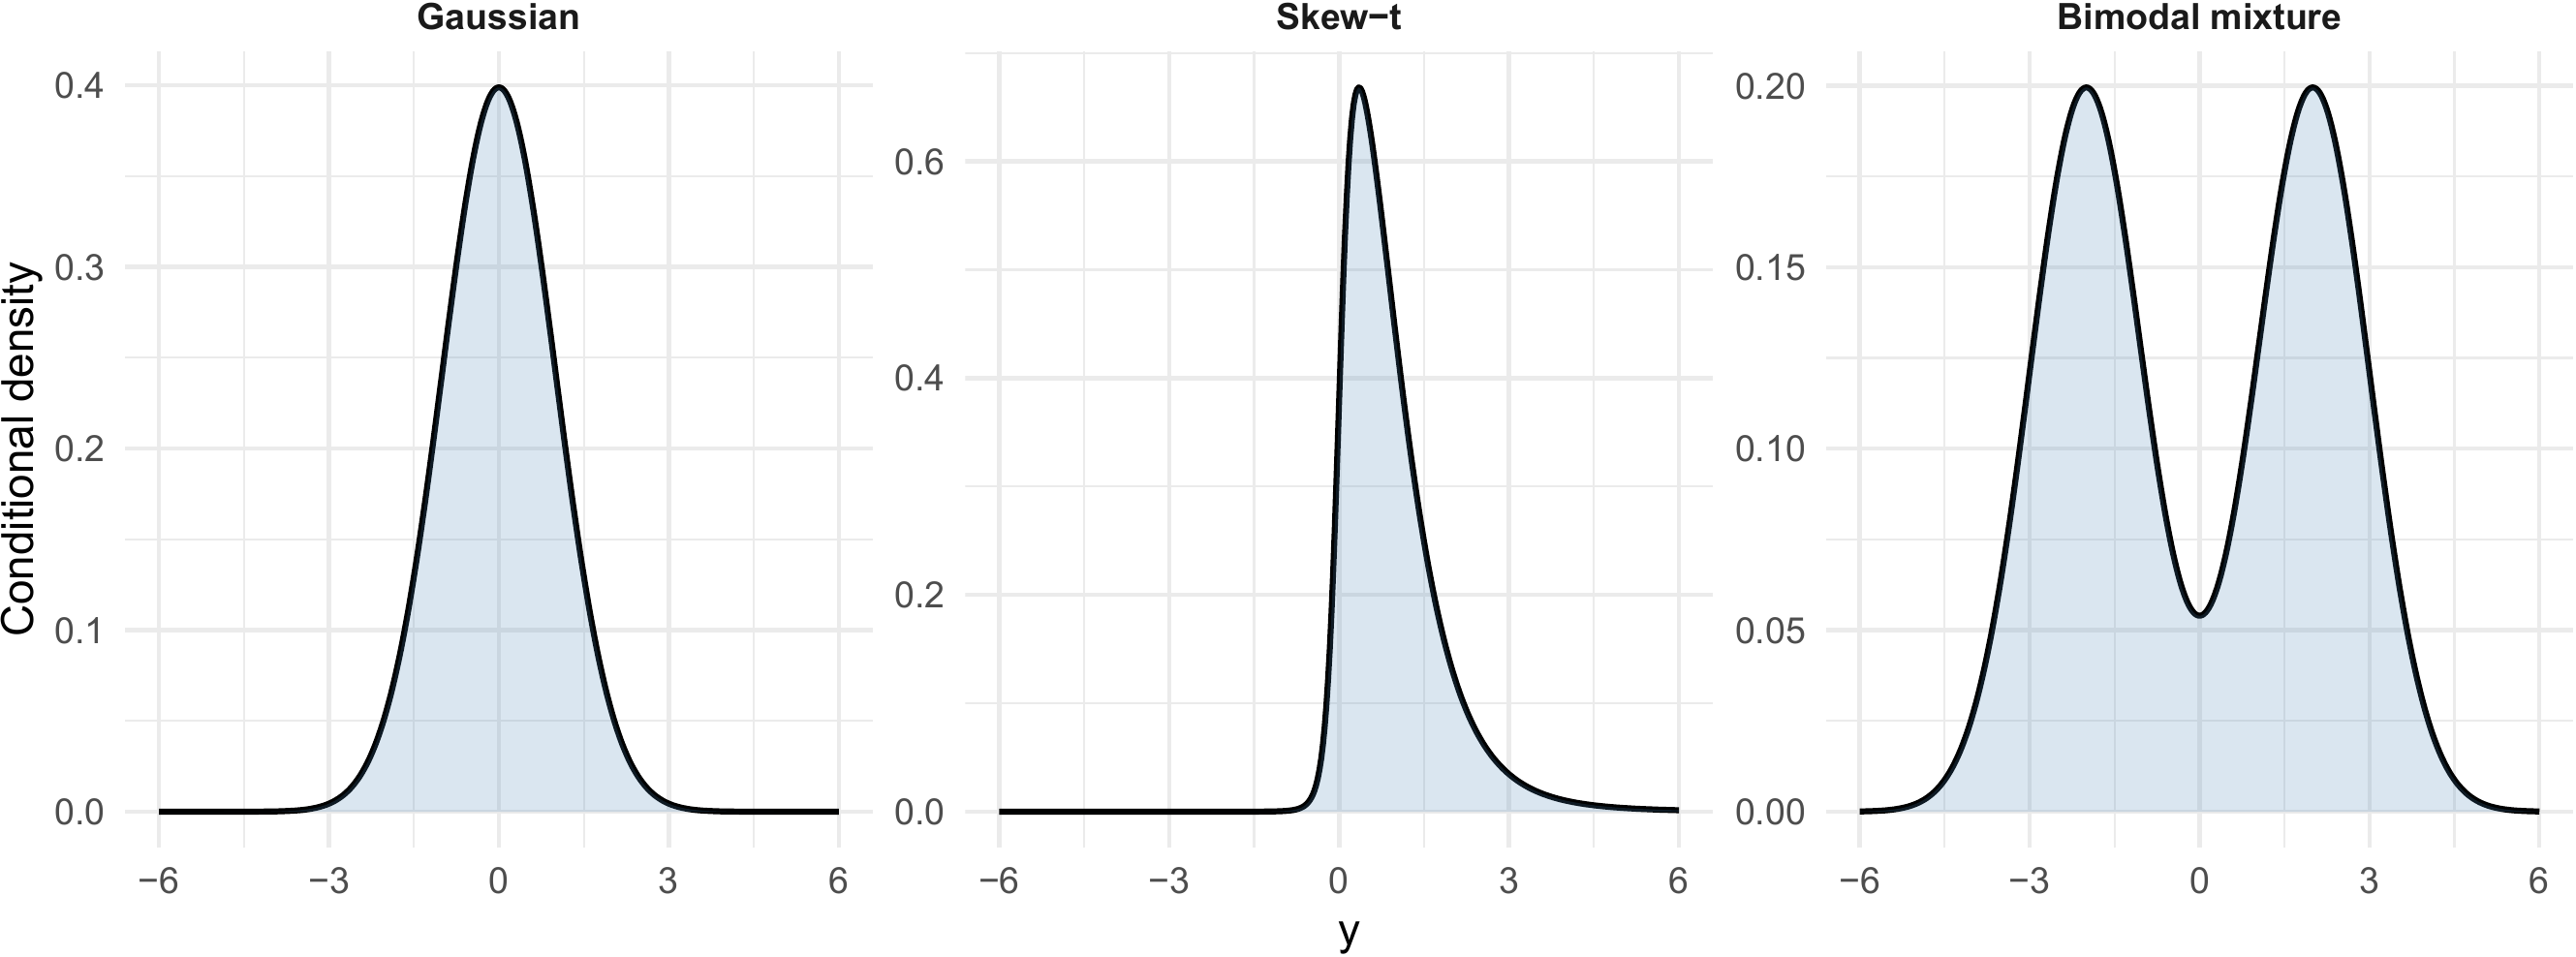
\includegraphics[width=\textwidth]{fig_dgp_densities.png}}
\end{figure}

\section{Design}
\label{sec:mc-design}

The Monte Carlo experiment consists of $R = 100$ independent replications. In each replication, a sample of $T = 250$ observations is drawn from the DGP defined in Section~\ref{sec:dgps}, chosen to be similar to the effective sample size in the empirical application. On each simulated sample, quantile regressions of $y_t$ on a constant and $x_t$ are estimated at the baseline grid of $k = 19$ quantile levels described in Section~\ref{sec:qr}, yielding an estimated conditional quantile function at each observed value of the covariate. The two smoothing procedures described in Sections~\ref{subsec:skewt} and~\ref{subsec:mpz}, the parametric skew-$t$ of \textcite{adrian2019vulnerable} and the semi-parametric piecewise-linear procedure of \textcite{mitchell2024constructing}, are then applied to the estimated quantile function to produce a conditional density estimate at a fixed evaluation point.

The evaluation point is $x^* = 0$. For the bimodal DGP, this gives $\pi(x^*) = 0.5$, so the two mixture components receive equal weight. The common evaluation point makes the results directly comparable across DGPs. The metrics therefore measure performance for the same covariate value rather than averaging over different conditional densities.

We use $R=100$ replications because the skew-$t$ fitting procedure is computationally expensive. Each application of the skew-$t$ smoother requires numerical minimization of a criterion function whose evaluation itself involves numerical inversion of the skew-$t$ distribution function. The bounded optimization is run from three starting values per fit to account for local minima, which multiplies the cost accordingly; with $R = 100$ replications and one skew-$t$ fit per replication, the total cost is manageable.

\section{Evaluation metrics}
\label{sec:mc-metrics}

The accuracy of each smoother's estimated conditional density at the evaluation point $x^* = 0$ is assessed using two complementary metrics. The first is the mean integrated squared error (MISE) between the estimated density $\hat{f}(\cdot \mid x^*)$ and the true density $f(\cdot \mid x^*)$, defined as
\[
\text{MISE} = \int_{-\infty}^{\infty} \bigl(\hat{f}(y \mid x^*) - f(y \mid x^*)\bigr)^2 \, dy,
\]
which is computed numerically by trapezoidal integration on a dense grid of values of $y$. The MISE captures the average squared discrepancy between the estimated and true densities across the entire real line, and is thus a symmetric, unweighted measure of overall fit. The second metric is the log-score, defined as the value of the log estimated density at a random draw from the true conditional distribution:
\[
\text{LogScore} = \log \hat{f}(y^\star \mid x^*), \qquad y^\star \sim f(\cdot \mid x^*).
\]
The log-score is a strictly proper scoring rule \parencite{gneiting2007strictly} that rewards estimated densities placing high probability mass at values likely under the true density; a higher log-score indicates a more accurate density estimate. For each replication, the log-score is averaged over $M = 100$ independent draws from the true conditional distribution to reduce Monte Carlo noise in the metric itself. The Monte Carlo study reports MISE and the log-score because the two metrics weight density errors differently. MISE measures the integrated squared distance between the estimated and true densities, whereas the log-score evaluates the predictive density at realized draws.

\section{Results}
\label{sec:mc-results}

\begin{table}[htbp]
	\ttabbox[\FBwidth]
	{\caption[Monte Carlo results]{Monte Carlo results across three data-generating processes. Mean MISE and log-score at the evaluation point $x^* = 0$, averaged over $R = 100$ replications with $T = 250$. Standard errors in parentheses. Lower MISE and higher log-score indicate better density estimation. Paired $t$-statistics test the null of equal performance between smoothers.}
	\label{tab:mc}}
	{\small
	\begin{tabular}{lcccc}
		\toprule
		& \multicolumn{2}{c}{MISE} & \multicolumn{2}{c}{Log-score} \\
		\cmidrule(lr){2-3} \cmidrule(lr){4-5}
		Smoother & Mean & SE & Mean & SE \\
		\midrule
		\multicolumn{5}{l}{\textit{Gaussian}} \\
		Skew-$t$ (ABG) & 0.0027 & (0.0003) & $-$1.4400 & (0.0077) \\
		Piecewise-linear (MPZ) & 0.0038 & (0.0002) & $-$1.4324 & (0.0079) \\
		Difference (Skew-$t$ $-$ MPZ) & $-$0.0011 & $t = -4.22$ & $-$0.0076 & $t = -0.72$ \\
		\addlinespace
		\multicolumn{5}{l}{\textit{Skew-$t$}} \\
		Skew-$t$ (ABG) & 0.0094 & (0.0007) & $-$1.1168 & (0.0113) \\
		Piecewise-linear (MPZ) & 0.0076 & (0.0004) & $-$1.7787 & (0.2039) \\
		Difference (Skew-$t$ $-$ MPZ) & 0.0018 & $t = 2.22$ & 0.6619 & $t = 3.24$ \\
		\addlinespace
		\multicolumn{5}{l}{\textit{Bimodal mixture}} \\
		Skew-$t$ (ABG) & 0.0530 & (0.0005) & $-$2.2669 & (0.0056) \\
		Piecewise-linear (MPZ) & 0.0329 & (0.0008) & $-$2.1866 & (0.0067) \\
		Difference (Skew-$t$ $-$ MPZ) & 0.0201 & $t = 29.22$ & $-$0.0802 & $t = -8.96$ \\
		\bottomrule
	\end{tabular}}
\end{table}

Table~\ref{tab:mc} reports the Monte Carlo performance metrics across the three data-generating processes. Differences are computed as skew-$t$ minus MPZ, so a negative MISE $t$-statistic and a positive log-score $t$-statistic both favor the skew-$t$. Under the symmetric Gaussian benchmark the skew-$t$ attains a lower MISE ($t = -4.22$) while the log-score difference is negligible ($t = -0.72$). Under the skew-$t$ DGP, the two metrics disagree. The parametric procedure attains a substantially higher log-score,
\[
t = 3.24,
\]
as expected when its parametric assumption holds exactly. However, MPZ attains a lower MISE,
\[
t = 2.22.
\]
The two metrics differ because they weight density errors differently. The log-score is evaluated at draws from the true density and therefore places greater weight on the region where probability mass actually falls, whereas MISE weights the whole real line equally and penalizes the skew-$t$ distribution's heavier fitted tails. The bimodal mixture reverses the ranking decisively: the semi-parametric MPZ smoother cuts MISE by roughly 38 percent relative to the skew-$t$ ($t = 29.22$) and attains a higher log-score ($t = -8.96$).

\begin{figure}[htbp]
	\ffigbox[\FBwidth]{%
		\caption[Representative Monte Carlo replication]{Representative Monte Carlo replication for each DGP. True conditional density (black) versus estimated densities under the skew-$t$ smoother (red) and the piecewise-linear smoother (blue). The Gaussian DGP is recovered well by both smoothers. The skew-$t$ DGP is recovered well by both, with the skew-$t$ smoother having a slight parametric advantage. The bimodal DGP is recovered only by the piecewise-linear smoother; the skew-$t$ collapses the bimodality into a single unimodal density.}%
		\label{fig:mc-rep}%
	}
	{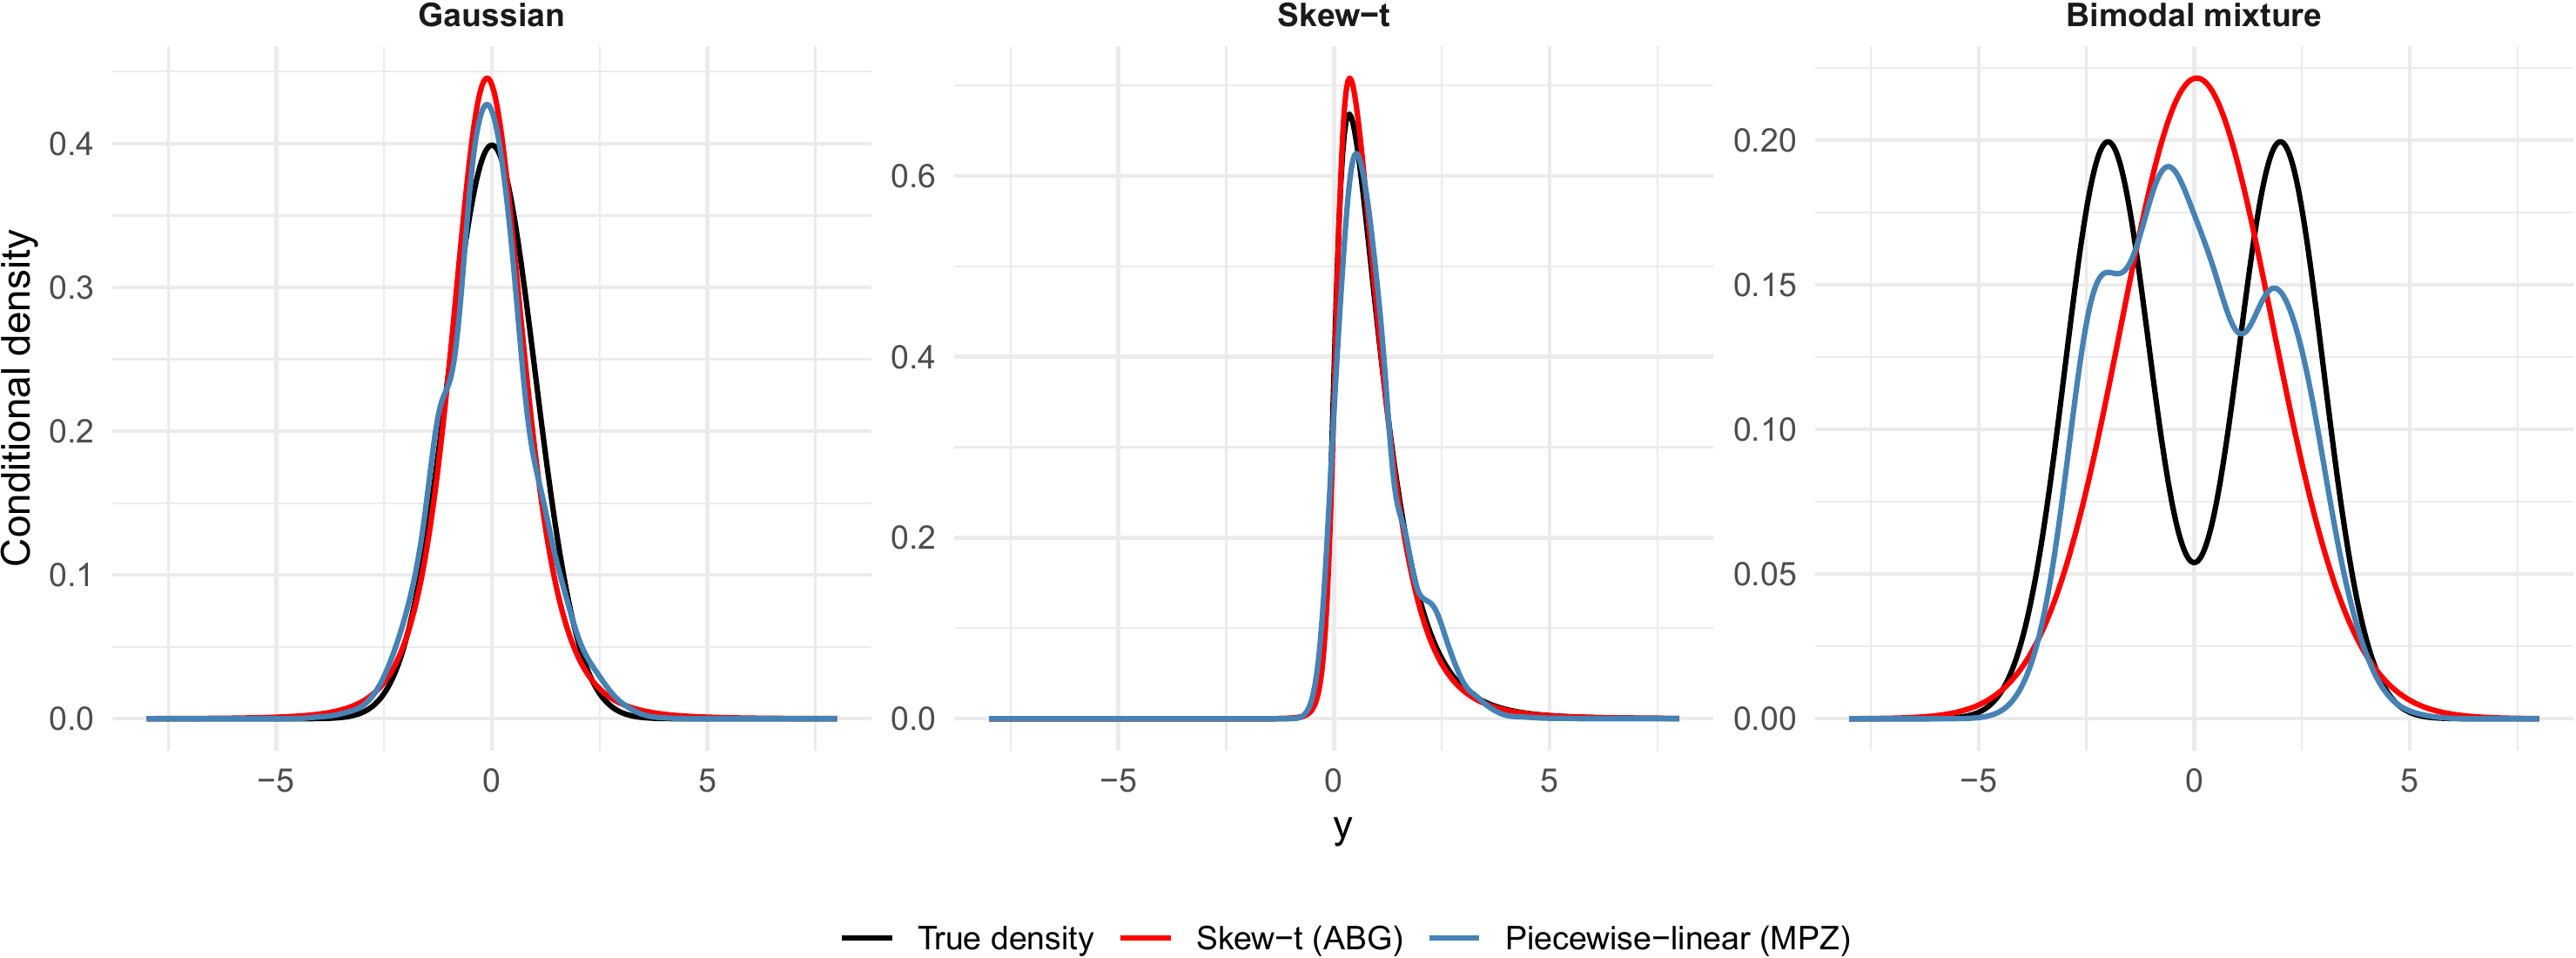
\includegraphics[width=\textwidth]{fig_mc_replication.png}}
\end{figure}

Figure~\ref{fig:mc-rep} visually illustrates these dynamics for a representative simulation draw. In the Gaussian panel, all three curves overlap closely, confirming that neither smoother introduces noticeable distortion when the underlying density is symmetric and unimodal. In the skew-$t$ panel, both methods track the true distribution, though MPZ exhibits minor piecewise-linear approximation noise along the right tail. The bimodal panel shows the main difference between the two procedures: the parametric skew-$t$ smoother collapses the two modes into a single, overly broad unimodal peak positioned between them. In contrast, the MPZ smoother successfully captures both primary peaks and the central trough with some finite-sample variation.

Under the symmetric Gaussian the parametric smoother is more accurate on MISE. Under the skew-$t$ the two metrics disagree. Under the bimodal mixture the semi-parametric smoother wins on both metrics, with by far the largest test statistics in the table. The skew-$t$ matches or beats MPZ on at least one metric for both unimodal processes while using only four of the nineteen estimated quantiles. This shows that using only four quantiles does not prevent the skew-$t$ smoother from performing well when the density is unimodal. However, MPZ uses fifteen additional quantiles in the bimodal case, so the information difference remains a potential contributor to its advantage.

The frequency with which the skew-$t$ fit reaches a parameter bound varies sharply across DGPs: 38 of 100 replications under the Gaussian, 23 under the skew-$t$, and 86 under the bimodal mixture. When the true density is bimodal, the estimated quantiles are, in the large majority of replications, not well matched by any skew-$t$ within the admissible parameter range.

%----------
%	4. EMPIRICAL APPLICATION
%----------

\chapter{Empirical Application}
\label{ch:empirical}

The empirical application follows \textcite{adrian2019vulnerable} in taking one-quarter-ahead US real GDP growth as the target variable and in using US macroeconomic data as the source of conditioning information. The two central departures from ABG are, first, the replacement of the National Financial Conditions Index by principal-components factors extracted from a large macroeconomic panel, and second, the systematic comparison of alternative smoothing procedures in the mapping from estimated quantiles to conditional density. The chapter is organized as follows. Section~\ref{sec:data} describes the FRED-QD data. Section~\ref{sec:factors-est} reports the results of the factor extraction step. Section~\ref{sec:quantiles} presents the estimated factor-augmented quantile regressions. Section~\ref{sec:densities} compares the conditional densities obtained under alternative smoothing procedures for a set of representative dates. Section~\ref{sec:oos} reports an out-of-sample evaluation of both smoothers' density forecasts.

\section{Data}
\label{sec:data}

The data source is the FRED-QD quarterly macroeconomic database maintained by the Federal Reserve Bank of St.~Louis \parencite{mccracken2020fredqd}. The March 2026 vintage contains 245 quarterly time series observed from 1959 Q1 through 2025 Q4, a total of 268 quarterly observations spanning the entire post-war US business cycle including nine NBER-dated recessions. The vintage is fixed to ensure reproducibility.

The dataset is distributed as a comma-separated file with two rows of metadata. The first metadata row indicates, for each series, whether it is to be included in the factor-estimation panel. The second metadata row provides the transformation code recommended by the dataset authors to induce stationarity, using the scheme in which code 1 denotes the level, code 2 the first difference, code 5 the first difference of the natural logarithm, and code 6 the second difference of the natural logarithm. All series are transformed according to these recommendations.

The target variable is real GDP growth, constructed from series GDPC1 (real Gross Domestic Product) as four hundred times the first difference of the natural logarithm, giving quarterly growth at annualized rates. This transformation follows both the recommendation of the FRED-QD authors (transformation code 5 for GDPC1) and the convention adopted by ABG. GDPC1 is complete over the full sample and requires no imputation.

\section{Estimated factors}
\label{sec:factors-est}

The factor-estimation panel is constructed from the subset of FRED-QD series that the dataset authors flag as intended for factor extraction. From this candidate set, we exclude the target variable GDPC1 to prevent contamination between the predictor and the predictand, and drop any series with more than twenty percent missing observations after transformation to stationarity. Of the 125 series flagged by the dataset authors for factor extraction, the target series GDPC1 is excluded, and 11 additional series are dropped for having more than 20 percent missing observations after transformation. The remaining 114 series form the factor-estimation panel; residual missing values are handled by column-wise mean imputation prior to standardization at the factor-estimation stage.

Principal-components factors are then extracted from the standardized panel, and the number of factors is selected by the $IC_{p2}$ criterion of \textcite{bai2002determining}. The criterion attains its minimum at $\hat{r} = 5$, so 5 factors are retained for use in the quantile regressions in Section~\ref{sec:quantiles}. Table~\ref{tab:variance} reports the share of panel variance explained by each of the first ten principal components. The first factor alone accounts for 22.4 percent of the variation in the panel, consistent with the well-known finding that a single dominant common factor captures much of the co-movement in US macroeconomic data. The 5 retained factors together explain 43.8 percent of the total variation in the panel.

\begin{table}[htbp]
	\ttabbox[\FBwidth]
	{\caption[Variance explained by the principal-components factors]{Share of panel variance explained by the first ten principal-components factors of the FRED-QD panel (2026-03 vintage, transformed series). The Bai-Ng $IC_{p2}$ criterion selects five factors.}
	\label{tab:variance}}
	{\small
	\begin{tabular}{lcc}
		\toprule
		Factor & Variance explained (\%) & Cumulative (\%) \\
		\midrule
		F1  & 22.40 & 22.40 \\
		F2  &  7.61 & 30.01 \\
		F3  &  6.17 & 36.18 \\
		F4  &  4.05 & 40.23 \\
		F5  &  3.56 & 43.79 \\
		F6  &  2.93 & 46.72 \\
		F7  &  2.60 & 49.32 \\
		F8  &  2.36 & 51.68 \\
		F9  &  2.22 & 53.90 \\
		F10 &  2.03 & 55.93 \\
		\bottomrule
	\end{tabular}}
\end{table}

Figure~\ref{fig:factors} plots the time series of the first four estimated factors, with NBER-dated recessions shaded. The first factor tracks a broad measure of real-activity fluctuation, with pronounced negative excursions during every post-war recession and a large movement during the COVID-19 contraction and rebound in 2020. The second and third factors capture additional cyclical dimensions, while the fourth is more idiosyncratic. These patterns are consistent with the interpretation of the leading principal components in FRED-based factor models as a real-activity factor followed by additional factors related to prices, financial conditions, and other secondary dimensions of macroeconomic variation.

\begin{figure}[htbp]
	\ffigbox[\FBwidth]{%
		\caption[Estimated principal-components factors]{First four estimated principal-components factors from the FRED-QD panel, 1959 Q3--2025 Q4. Shaded regions denote NBER-dated recessions.}%
		\label{fig:factors}%
	}
	{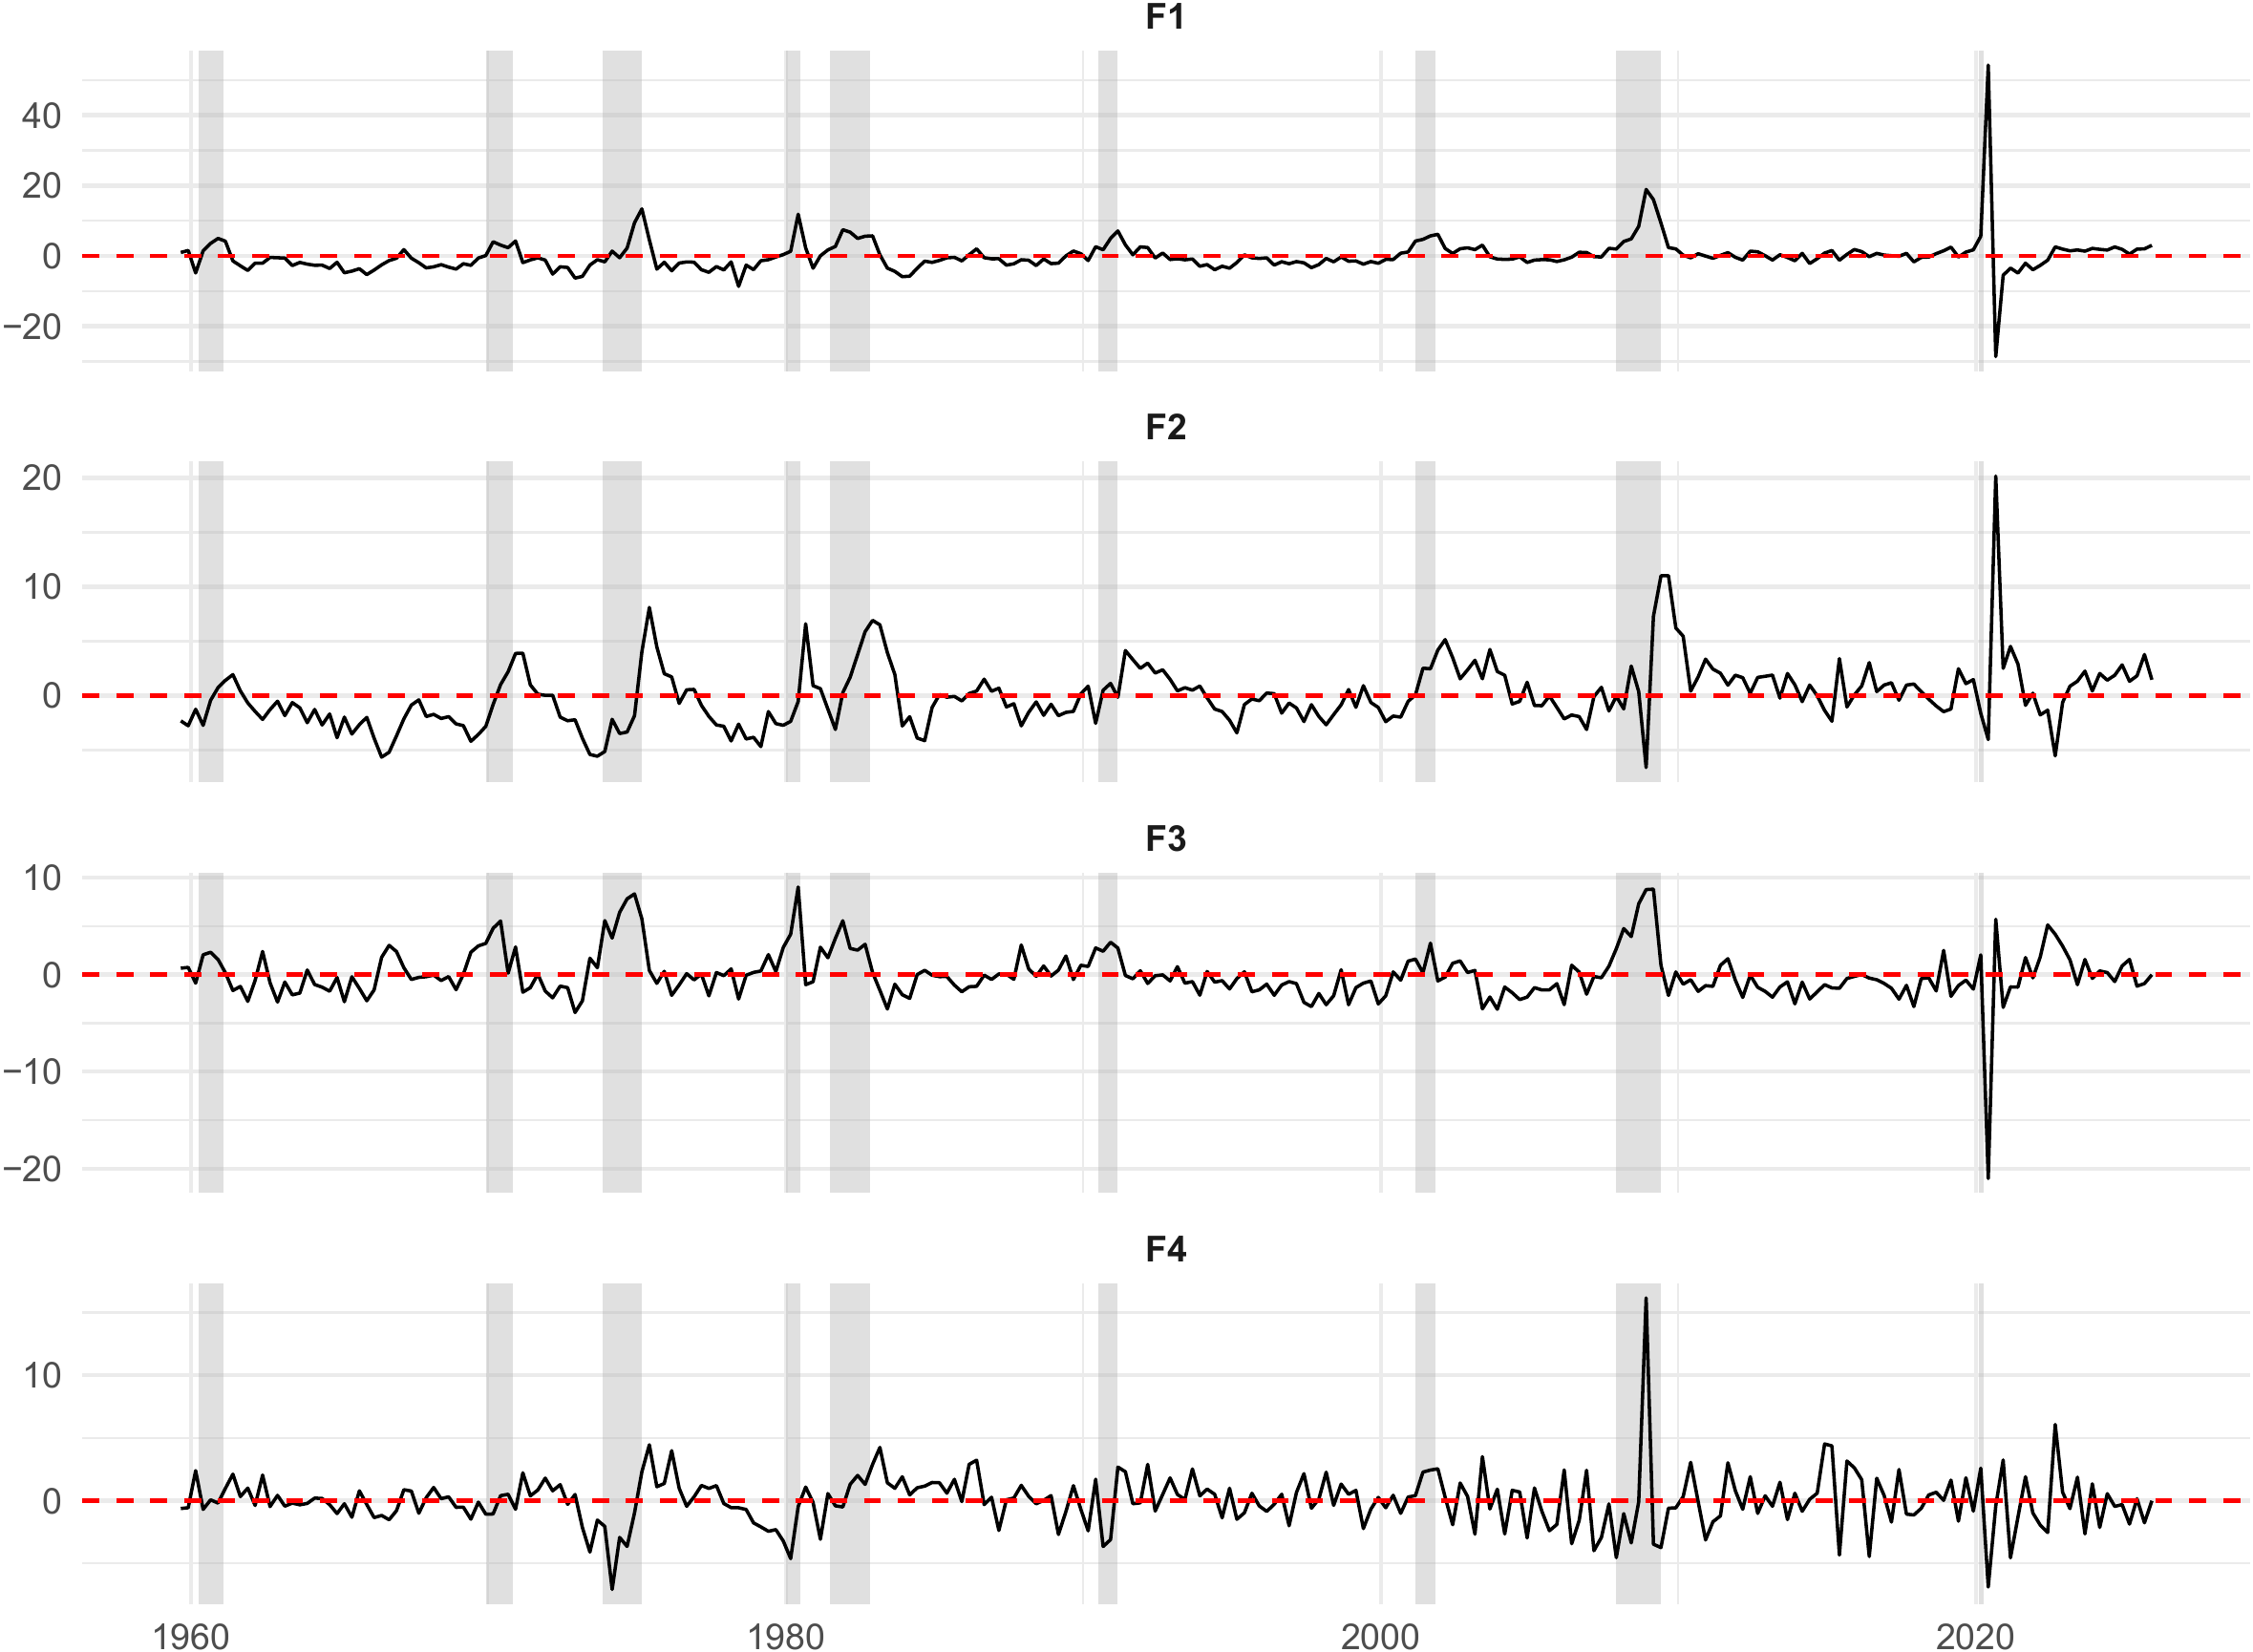
\includegraphics[width=\textwidth]{fig_factors.png}}
\end{figure}

\section{Estimated conditional quantiles}
\label{sec:quantiles}

Factor-augmented quantile regressions of one-quarter-ahead US GDP growth on the five extracted factors and one lag of GDP growth are estimated at the grid of nineteen quantile levels described in Section~\ref{sec:qr}. Each of the 19 quantile regressions is estimated separately on the full available sample, producing a set of 19 estimated conditional quantile forecasts at every date.

Figure~\ref{fig:coef} plots the estimated FA-QR coefficients across quantile levels, together with the corresponding OLS estimate (dashed red line) for comparison. Under the hypothesis that the conditional distribution of GDP growth differs from an ordinary linear regression only through location shifts, all quantile-regression slope coefficients should coincide with the OLS coefficient at every $\tau$; visible departures from a constant profile therefore indicate that the conditioning variables have differential effects across the conditional distribution. The coefficient on the lagged dependent variable is broadly stable across quantiles, whereas several factor coefficients vary substantially with $\tau$, consistent with the ABG finding that current macroeconomic and financial conditions have quantile-dependent effects on the distribution of future GDP growth.

\begin{figure}[htbp]
	\ffigbox[\FBwidth]{%
		\caption[Estimated FA-QR coefficients across quantile levels]{Estimated FA-QR coefficients across quantile levels. Solid line: quantile regression estimate. Dashed red line: OLS estimate. The coefficient on the lagged dependent variable is relatively stable across quantiles, while several factor coefficients vary, indicating differential impacts across the distribution.}%
		\label{fig:coef}%
	}
	{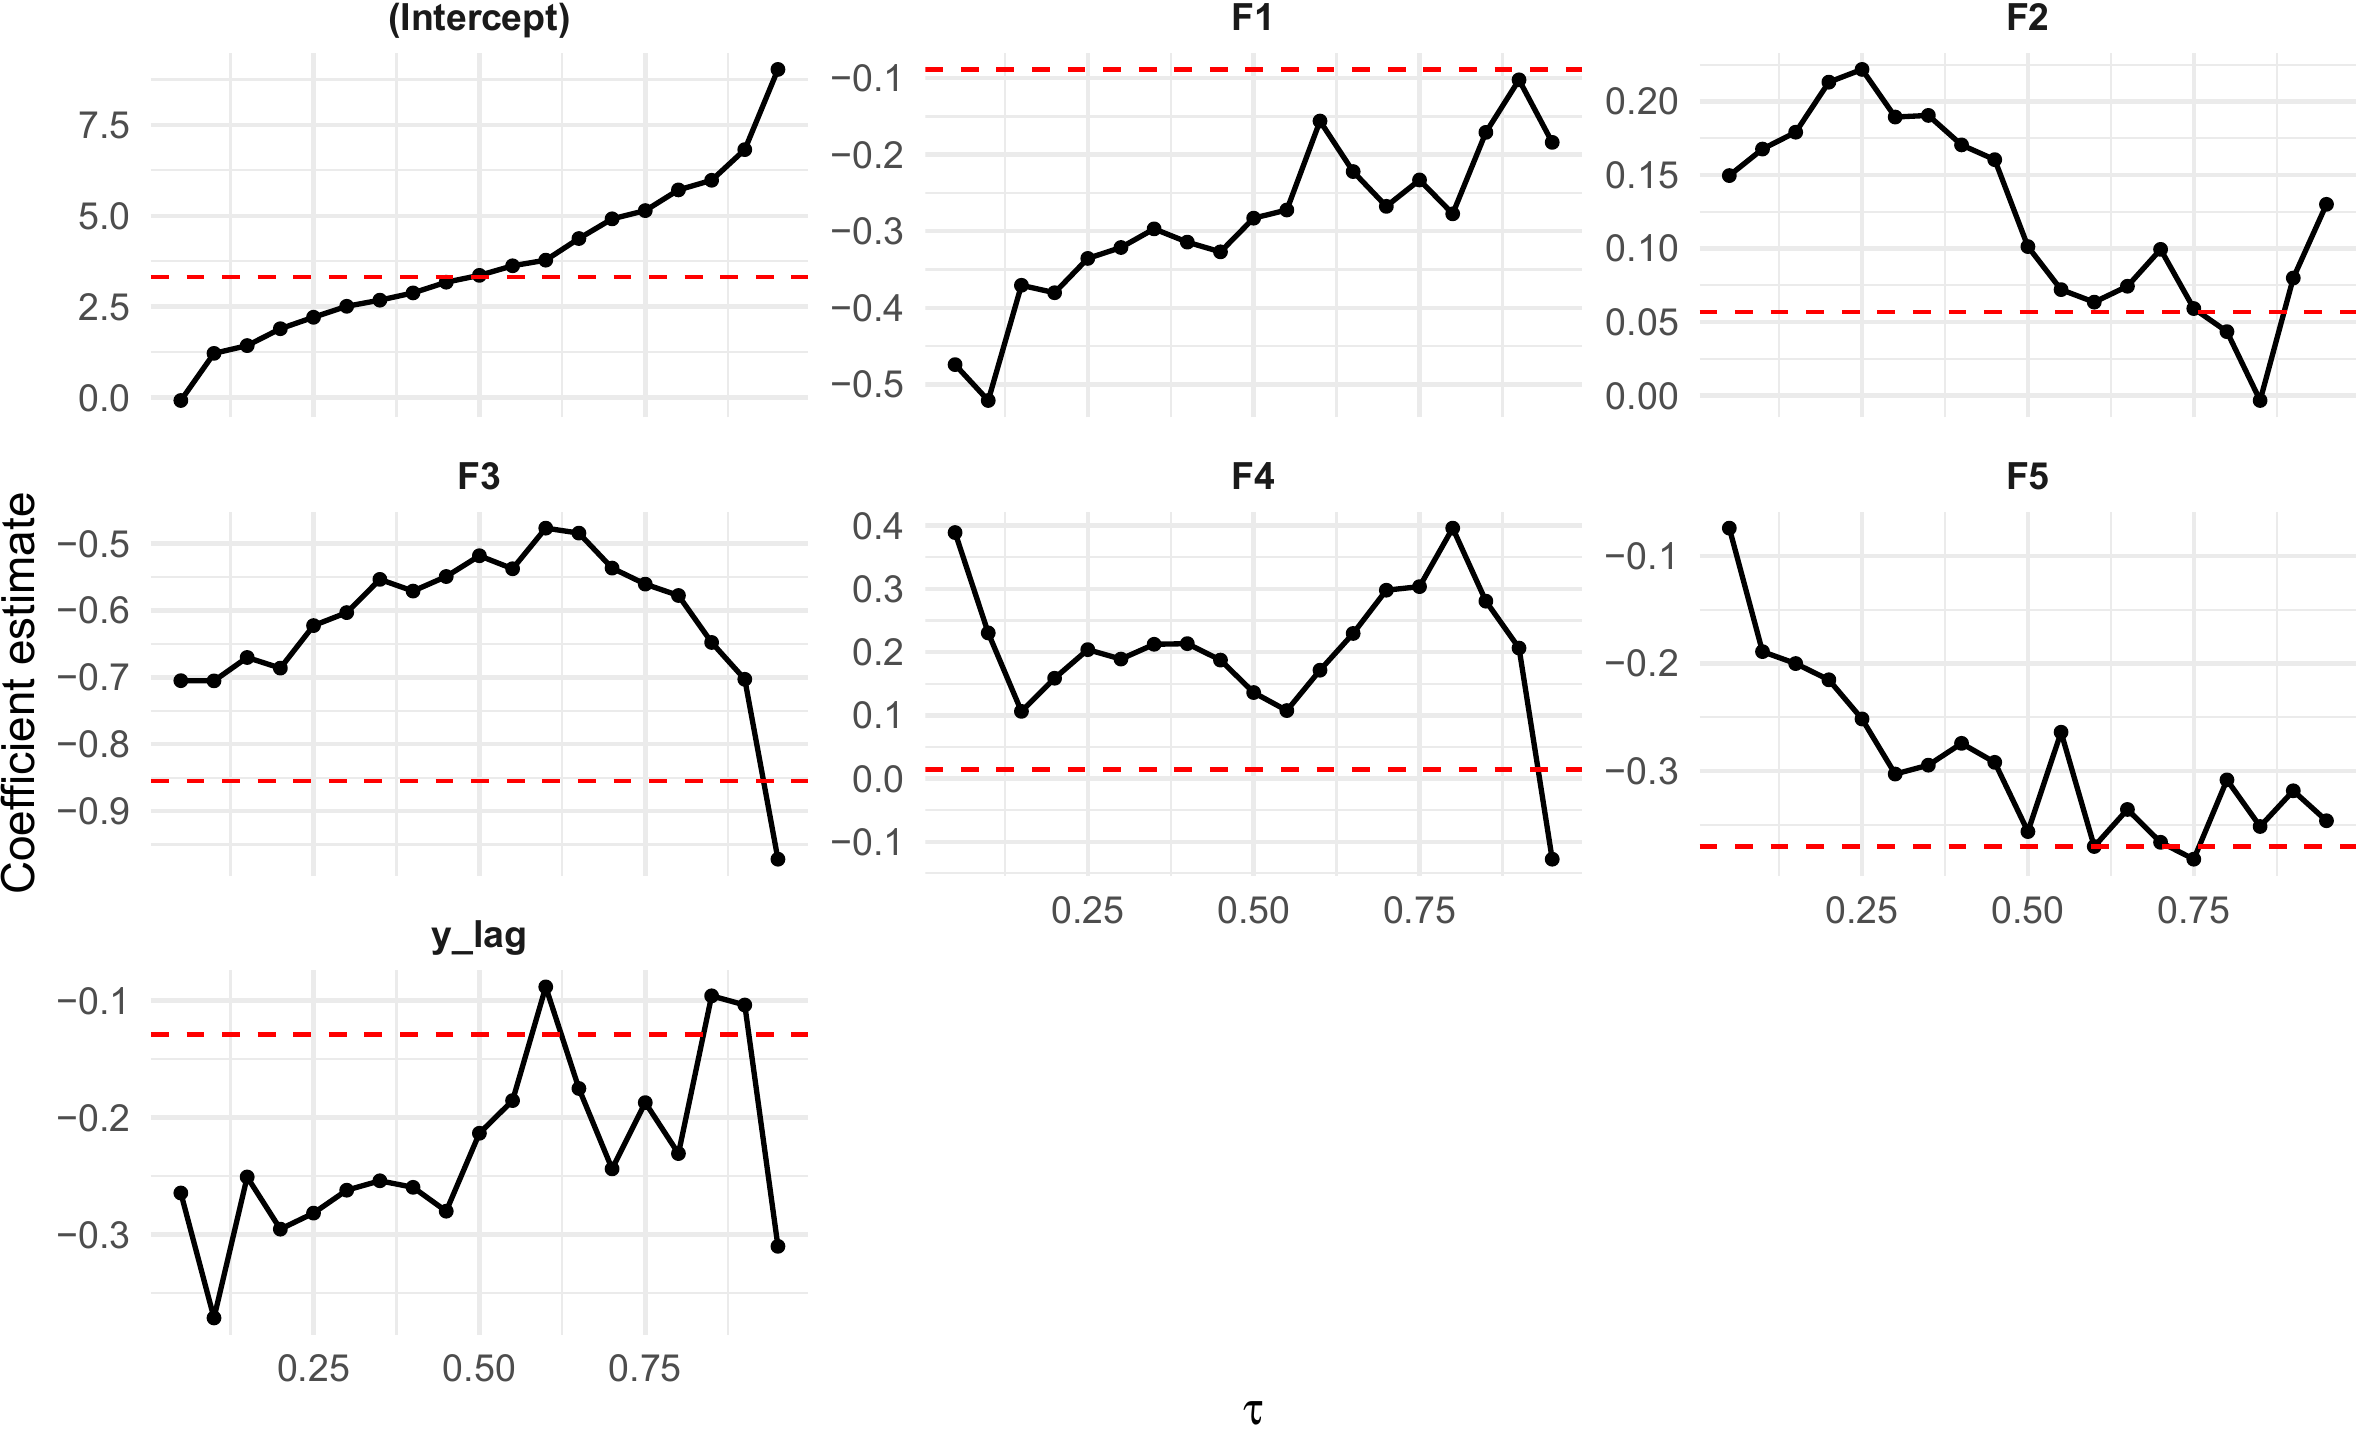
\includegraphics[width=\textwidth]{fig_faqr_coefficients.png}}
\end{figure}

Figure~\ref{fig:fan} presents the resulting conditional quantile forecasts as a fan chart over the sample period. The chart plots the estimated 5th, 25th, 50th, 75th, and 95th conditional quantiles of one-quarter-ahead GDP growth, together with the realized values. The lower quantiles exhibit greater time variation than the upper quantiles, with downward excursions during NBER-dated recessions, while the upper quantiles remain within a comparatively narrow range throughout the sample. This asymmetry between the time-series behavior of lower and upper conditional quantiles is the central Growth-at-Risk finding of ABG, and its replication with factor-based conditioning information suggests that the finding does not depend on the National Financial Conditions Index and also holds with factor-based conditioning.

\begin{figure}[htbp]
	\ffigbox[\FBwidth]{%
		\caption[Conditional quantiles of US GDP growth]{One-quarter-ahead conditional quantiles of US GDP growth from the FA-QR model, 1959--2025. Gray shading denotes NBER-dated recessions. Solid line: conditional median. Shaded bands: 25--75 and 5--95 quantile ranges. Dashed line: realized values. The lower quantiles exhibit substantially greater time variation than the upper quantiles.}%
		\label{fig:fan}%
	}
	{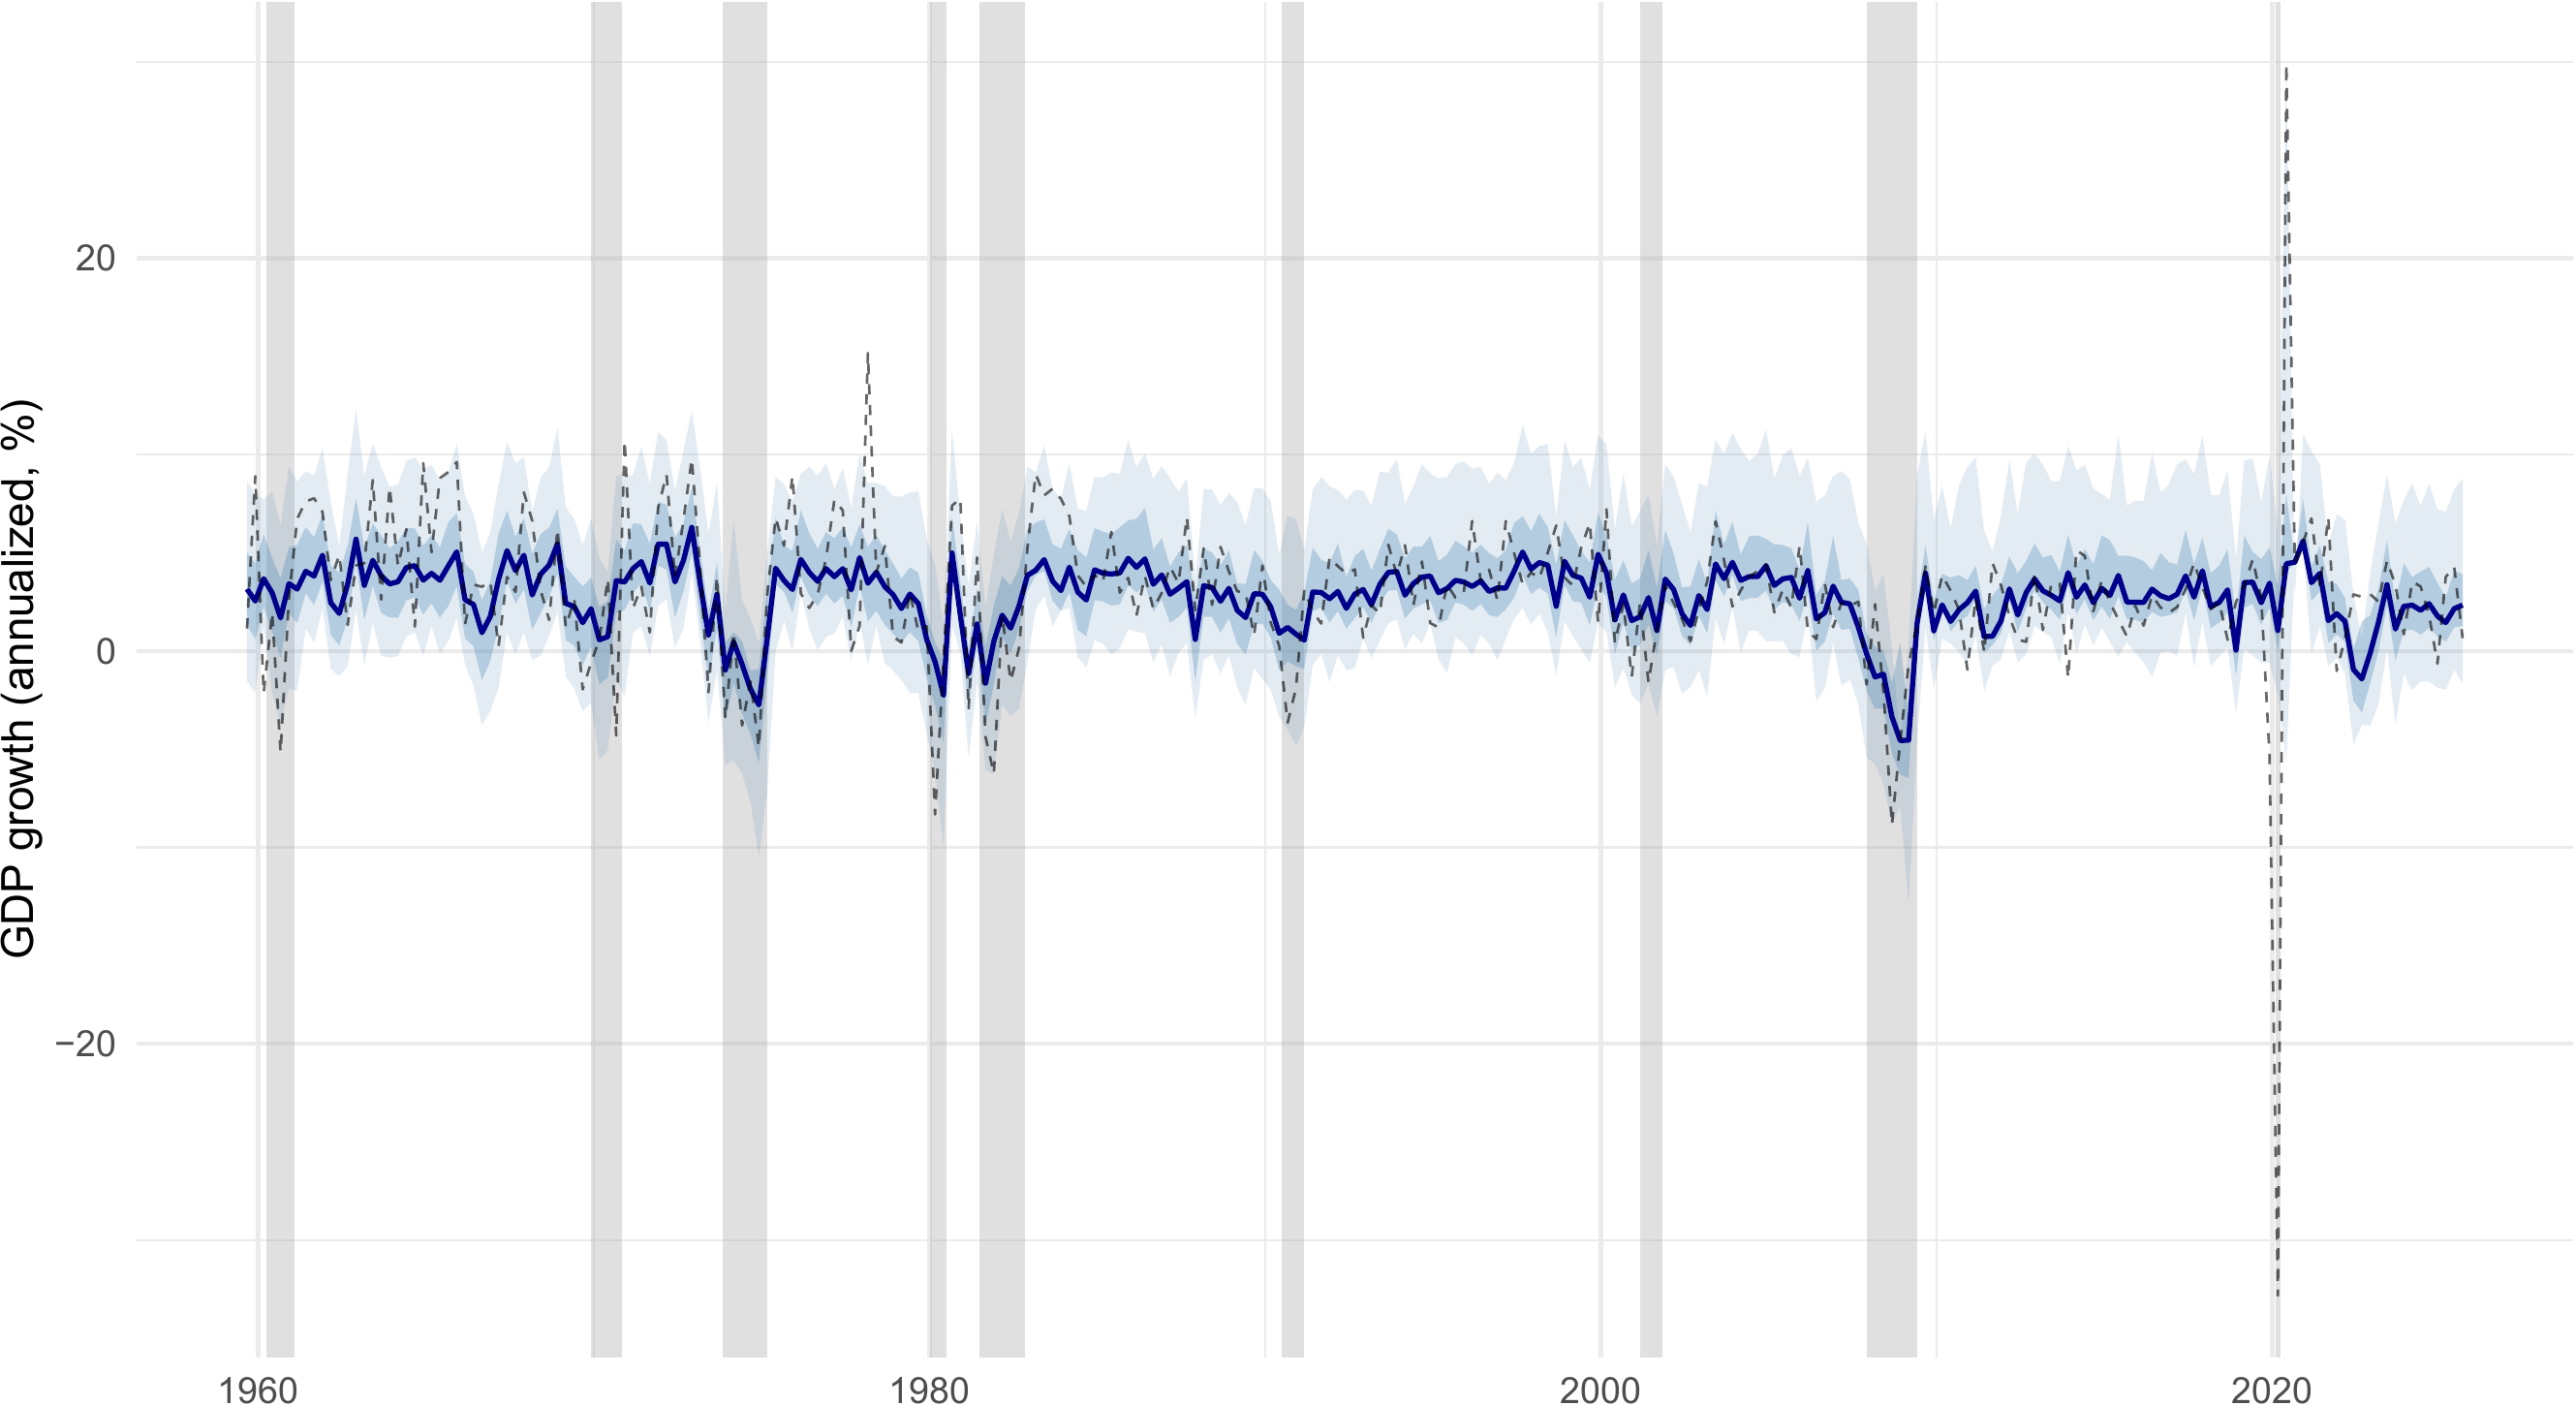
\includegraphics[width=\textwidth]{fig_quantile_fan.png}}
\end{figure}

\section{Estimated conditional densities}
\label{sec:densities}

The final step of the empirical application applies the smoothing procedures described in Section~\ref{sec:smoothing} to the estimated quantile forecasts of Section~\ref{sec:quantiles}, obtaining full conditional density forecasts of one-quarter-ahead GDP growth at each date. This section reports the resulting conditional densities under the parametric skew-$t$ procedure of ABG and the semi-parametric piecewise-linear procedure of Mitchell, Poon, and Zhu, for a set of four representative dates chosen to span distinct phases of the business cycle. Probability integral transforms are then computed in-sample for both smoothers. Section~\ref{sec:oos} reports an out-of-sample evaluation.

\begin{figure}[htbp]
	\ffigbox[\FBwidth]{%
		\caption[In-sample probability integral transforms]{In-sample probability integral transforms of one-quarter-ahead US GDP growth density forecasts. Left: empirical cumulative distribution function of the PIT values under each smoother, against the 45-degree line implied by correct calibration. Right: histogram of PIT values in twenty equal bins, with the dashed line marking the uniform density.}%
		\label{fig:pit-in}%
	}
	{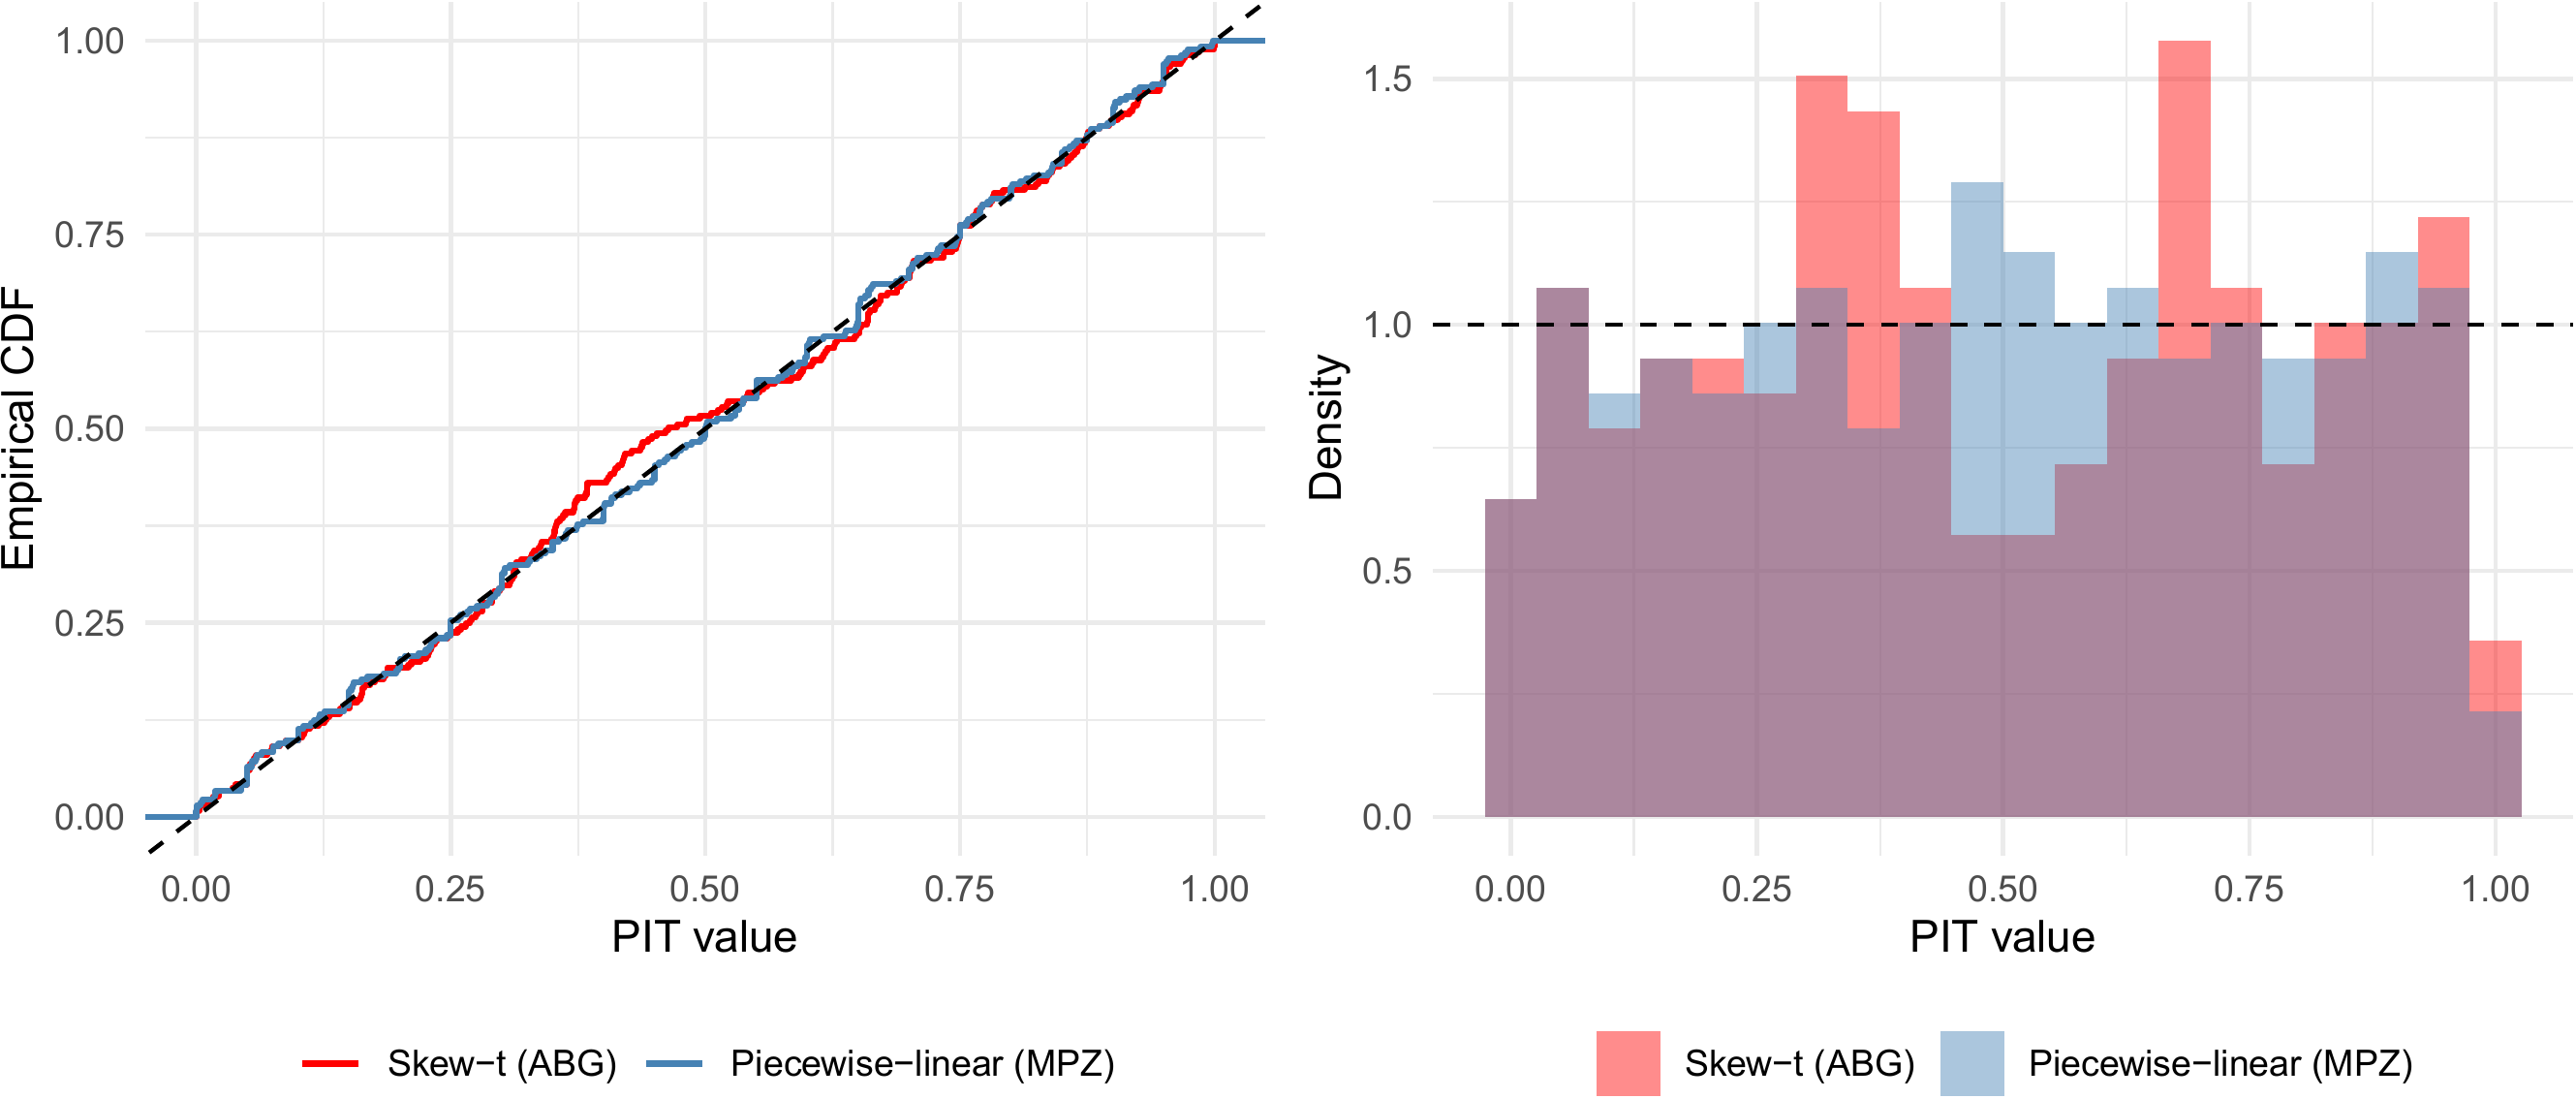
\includegraphics[width=\textwidth]{fig_pit_insample.png}}
\end{figure}

Figure~\ref{fig:densities} presents the estimated conditional density under the two smoothing procedures for four selected dates. Each density is a forecast made at the given date for growth in the following quarter. The 2006 Q2 date represents a period of expansion during the pre-crisis credit cycle. The 2008 Q4 date captures the acute phase of the financial crisis following the failure of Lehman Brothers. The 2014 Q4 date represents the middle of the post-crisis expansion. The 2020 Q2 date is the low point of the COVID-19 contraction, so its density is a forecast for the 2020 Q3 rebound.

\begin{figure}[htbp]
	\ffigbox[\FBwidth]{%
		\caption[Conditional densities at four selected dates]{Conditional density of one-quarter-ahead US GDP growth under skew-$t$ (ABG, red) and piecewise-linear (MPZ, blue) smoothing, for four selected dates. Dotted vertical line: realized value. The skew-$t$ density is by construction unimodal, while the MPZ density is free to exhibit multimodality.}%
		\label{fig:densities}%
	}
	{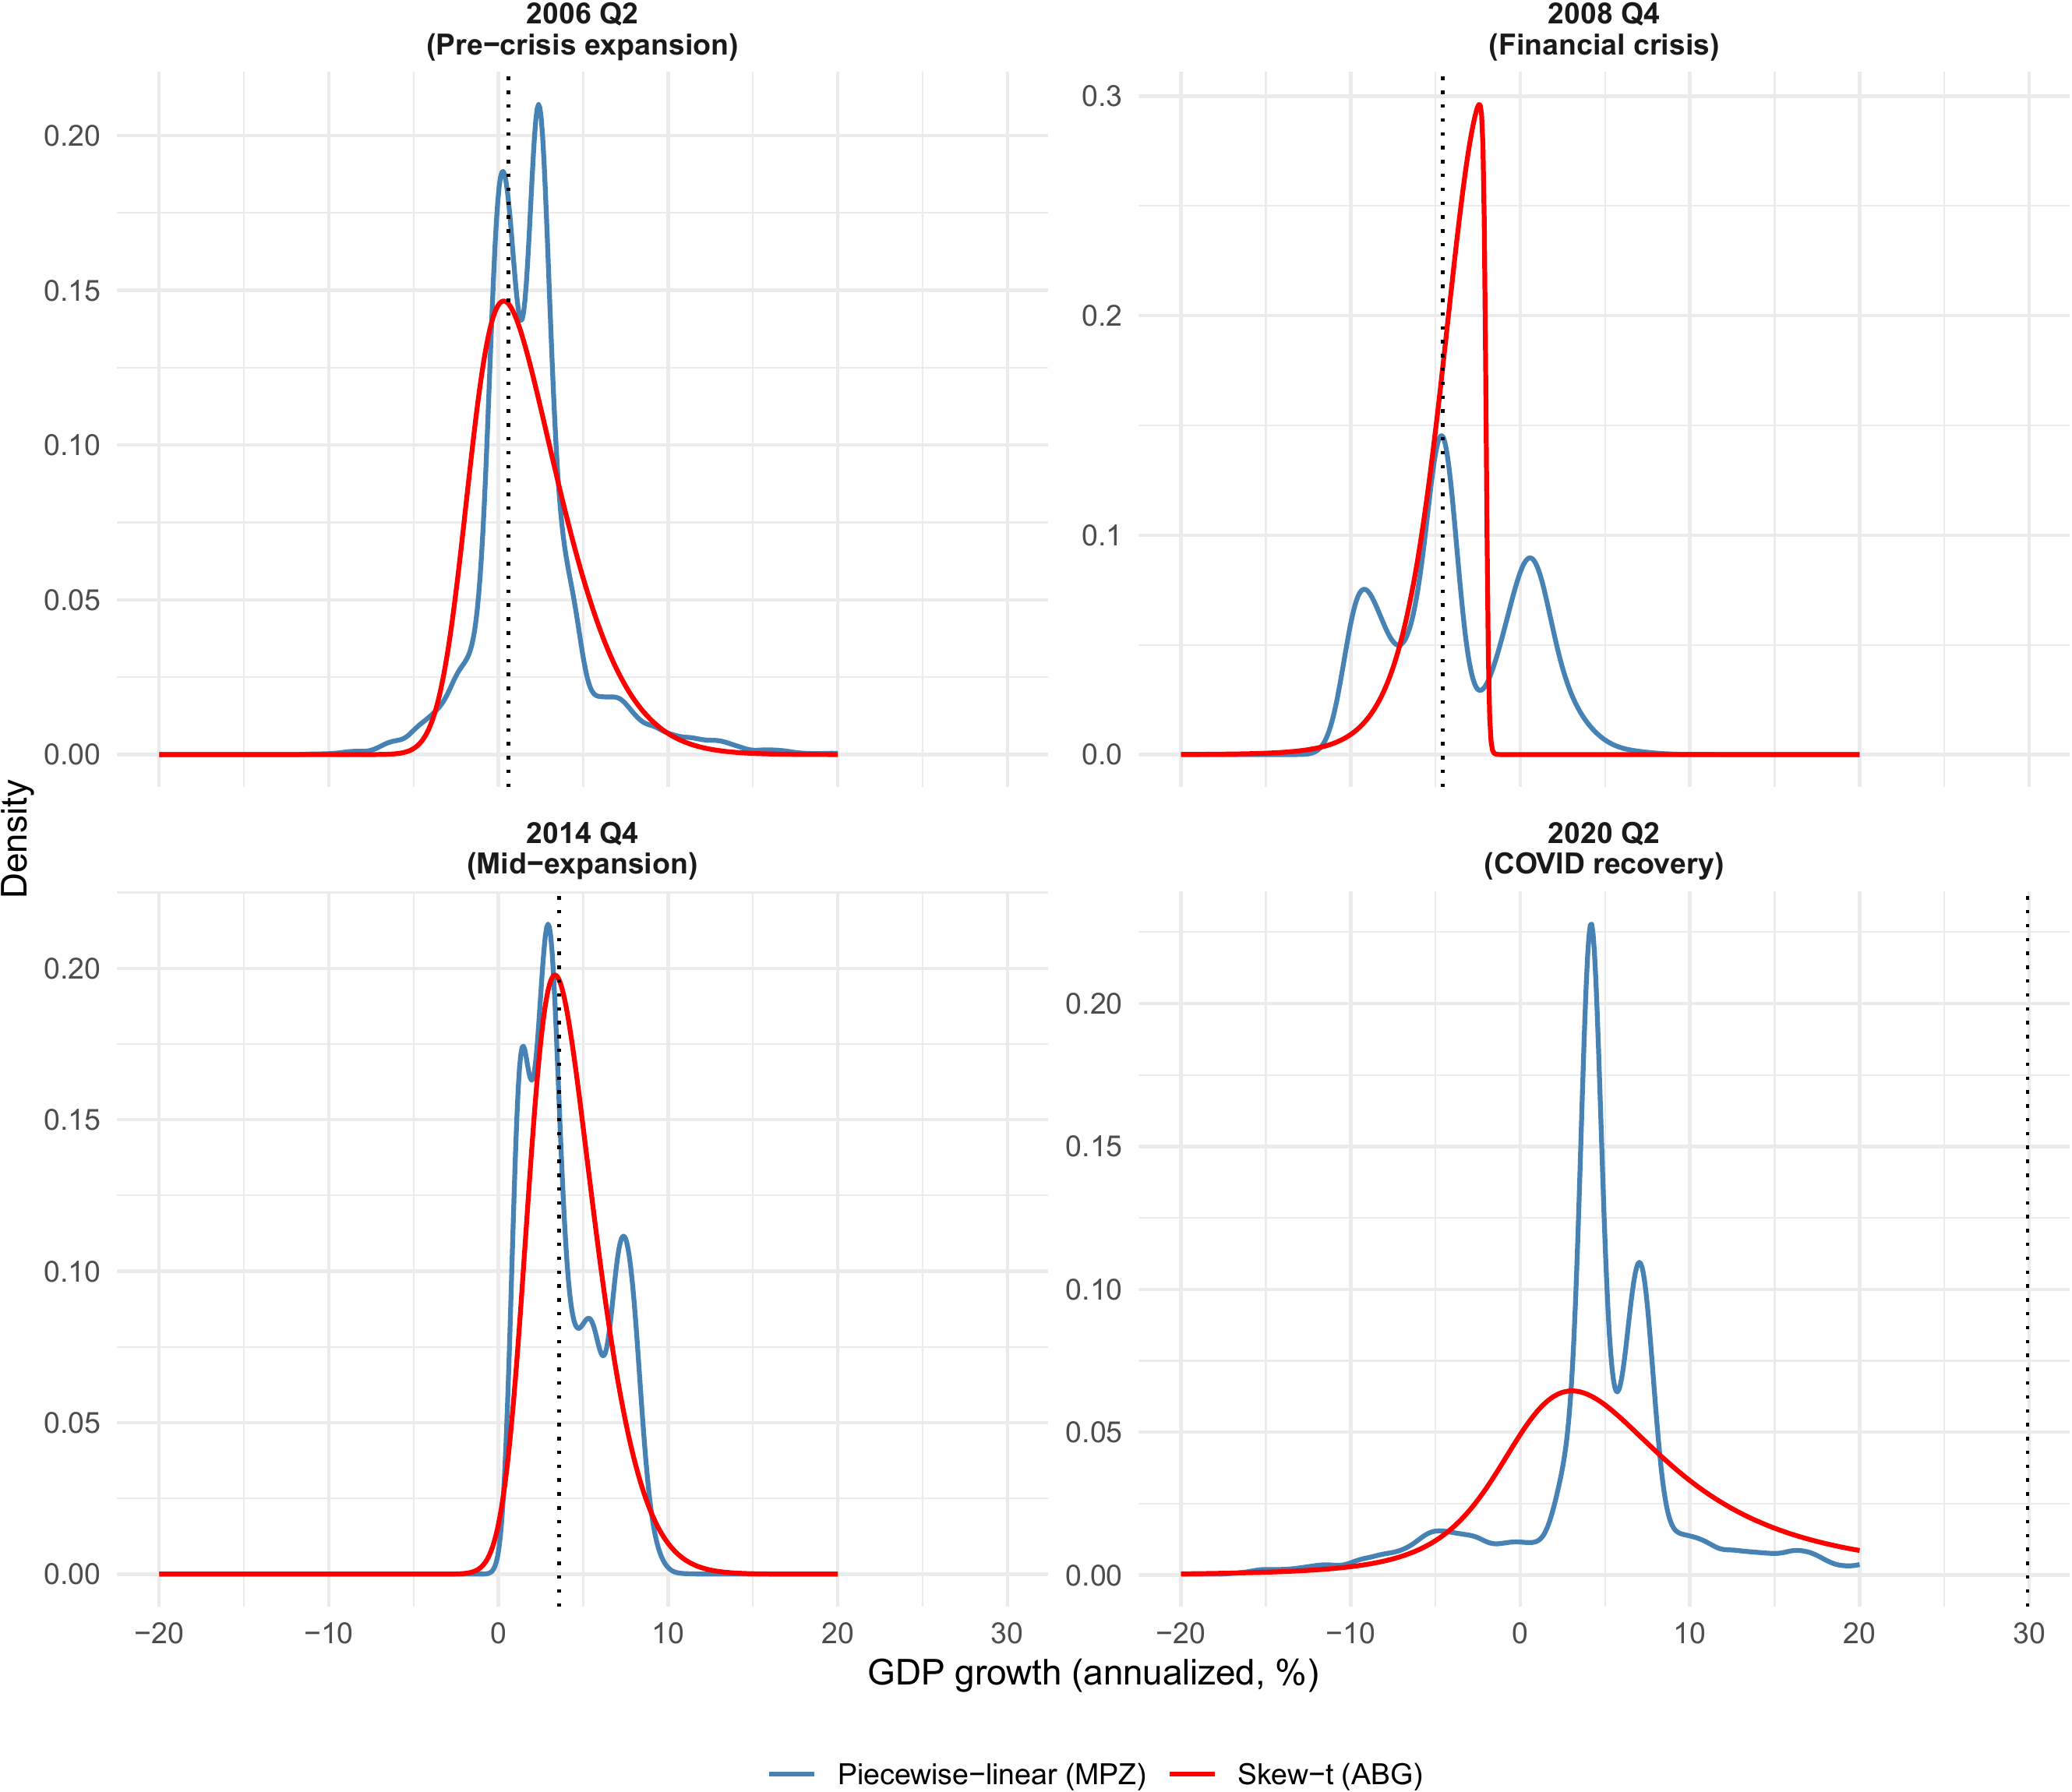
\includegraphics[width=\textwidth]{fig_density_dates.png}}
\end{figure}

Three patterns are visible in the comparison. First, during periods of stable expansion, the two smoothers produce nearly indistinguishable conditional densities. The 2006 Q2 panel shows the skew-$t$ and piecewise-linear densities essentially overlapping across the full range of the target variable, both exhibiting a single mode near the conditional median. At this date, the choice of smoother makes little difference.

Second, during the financial crisis, the two smoothers diverge substantially. The skew-$t$ density for 2008 Q4 is unimodal by construction, placing all of its mass in a single broad, negatively skewed distribution centered to the left of zero. The fitted shape parameter sits at the boundary of the permitted range, indicating that the estimated quantiles imply more negative skewness than the skew-$t$ family can accommodate within that range. The piecewise-linear density, by contrast, exhibits clear multimodality, with distinct modes on the far left of the distribution, near the conditional median, and in the right tail. This pattern replicates, within the factor-augmented setting, the multimodality finding of \textcite{mitchell2024constructing} for the original ABG specification, and suggests that the shape of the conditional density during crisis periods is substantively richer than a single skewed unimodal distribution can capture.

Third, even during mid-expansion periods such as 2014 Q4 and following extreme shocks such as the 2020 Q2 COVID rebound, the piecewise-linear smoother reveals secondary modal structure that the skew-$t$ smooths over. Section~\ref{sec:oos} checks whether these differences in shape affect forecast accuracy.

A pattern not visible in the figure is how often the skew-$t$ fit reaches a parameter bound. Across the 265 dates in the sample the bounds bind at 125 of them, or roughly 47 percent. Of these, 75 reach the upper limit on the degrees-of-freedom parameter, so that the fitted density is effectively a skew-normal; 44 reach the lower limit, implying tails heavier than the restriction permits; and 10 reach the limit on the shape parameter (a date can reach more than one bound). A binding bound means the estimated quantiles at that date cannot be matched by any skew-$t$ within the admissible range. Together, these results support the central premise of this thesis, namely that the choice of smoother is a substantive modeling decision with visible consequences for the estimated conditional density, particularly during periods of economic stress.

Figure~\ref{fig:pit-in} shows the in-sample PITs. These are of limited use for comparing calibration, because the quantile regressions are estimated on the same observations, so the share of outcomes below each fitted quantile is close to its nominal level by construction. This favors MPZ, which uses all nineteen fitted quantiles. Calibration is therefore compared out-of-sample in Section~\ref{sec:oos}.

\section{Out-of-sample density evaluation}
\label{sec:oos}

\begin{table}[htbp]
	\ttabbox[\FBwidth]
	{\caption[Out-of-sample density forecast evaluation]{Out-of-sample density forecast evaluation, 1990 Q2 to 2025 Q4 (143 quarters). Expanding estimation window with factors, quantile regressions and both smoothers re-estimated at every origin. Differences are skew-$t$ minus MPZ; $t$-statistics test the null of equal predictive accuracy.}
	\label{tab:oos}}
	{\small
	\begin{tabular}{lccccc}
		\toprule
		& Skew-$t$ & Piecewise-linear & & & \\
		Metric & (ABG) & (MPZ) & Difference & $t$-stat & $n$ \\
		\midrule
		CRPS             & 1.8169    & 1.8296    & $-$0.0127 & $-$0.89 & 143 \\
		CRPS, left tail  & 1.0679    & 1.0776    & $-$0.0097 & $-$0.86 & 143 \\
		CRPS, center     & 1.1043    & 1.1130    & $-$0.0088 & $-$0.97 & 143 \\
		CRPS, right tail & 0.7490    & 0.7520    & $-$0.0030 & $-$0.56 & 143 \\
		Log-score        & $-$2.4945 & $-$8.0478 & 5.5532    & 1.16    & 143 \\
		\bottomrule
	\end{tabular}}
\end{table}

\begin{figure}[htbp]
	\ffigbox[\FBwidth]{%
		\caption[Out-of-sample density forecast evaluation]{Out-of-sample density forecast evaluation. Top left: empirical CDF of the out-of-sample PIT values against the 45-degree line implied by correct calibration. Top right: histogram of PIT values in twenty equal bins. Bottom: cumulative difference in CRPS between the two smoothers over the evaluation window; an upward slope indicates the piecewise-linear smoother outperforming.}%
		\label{fig:oos}%
	}
	{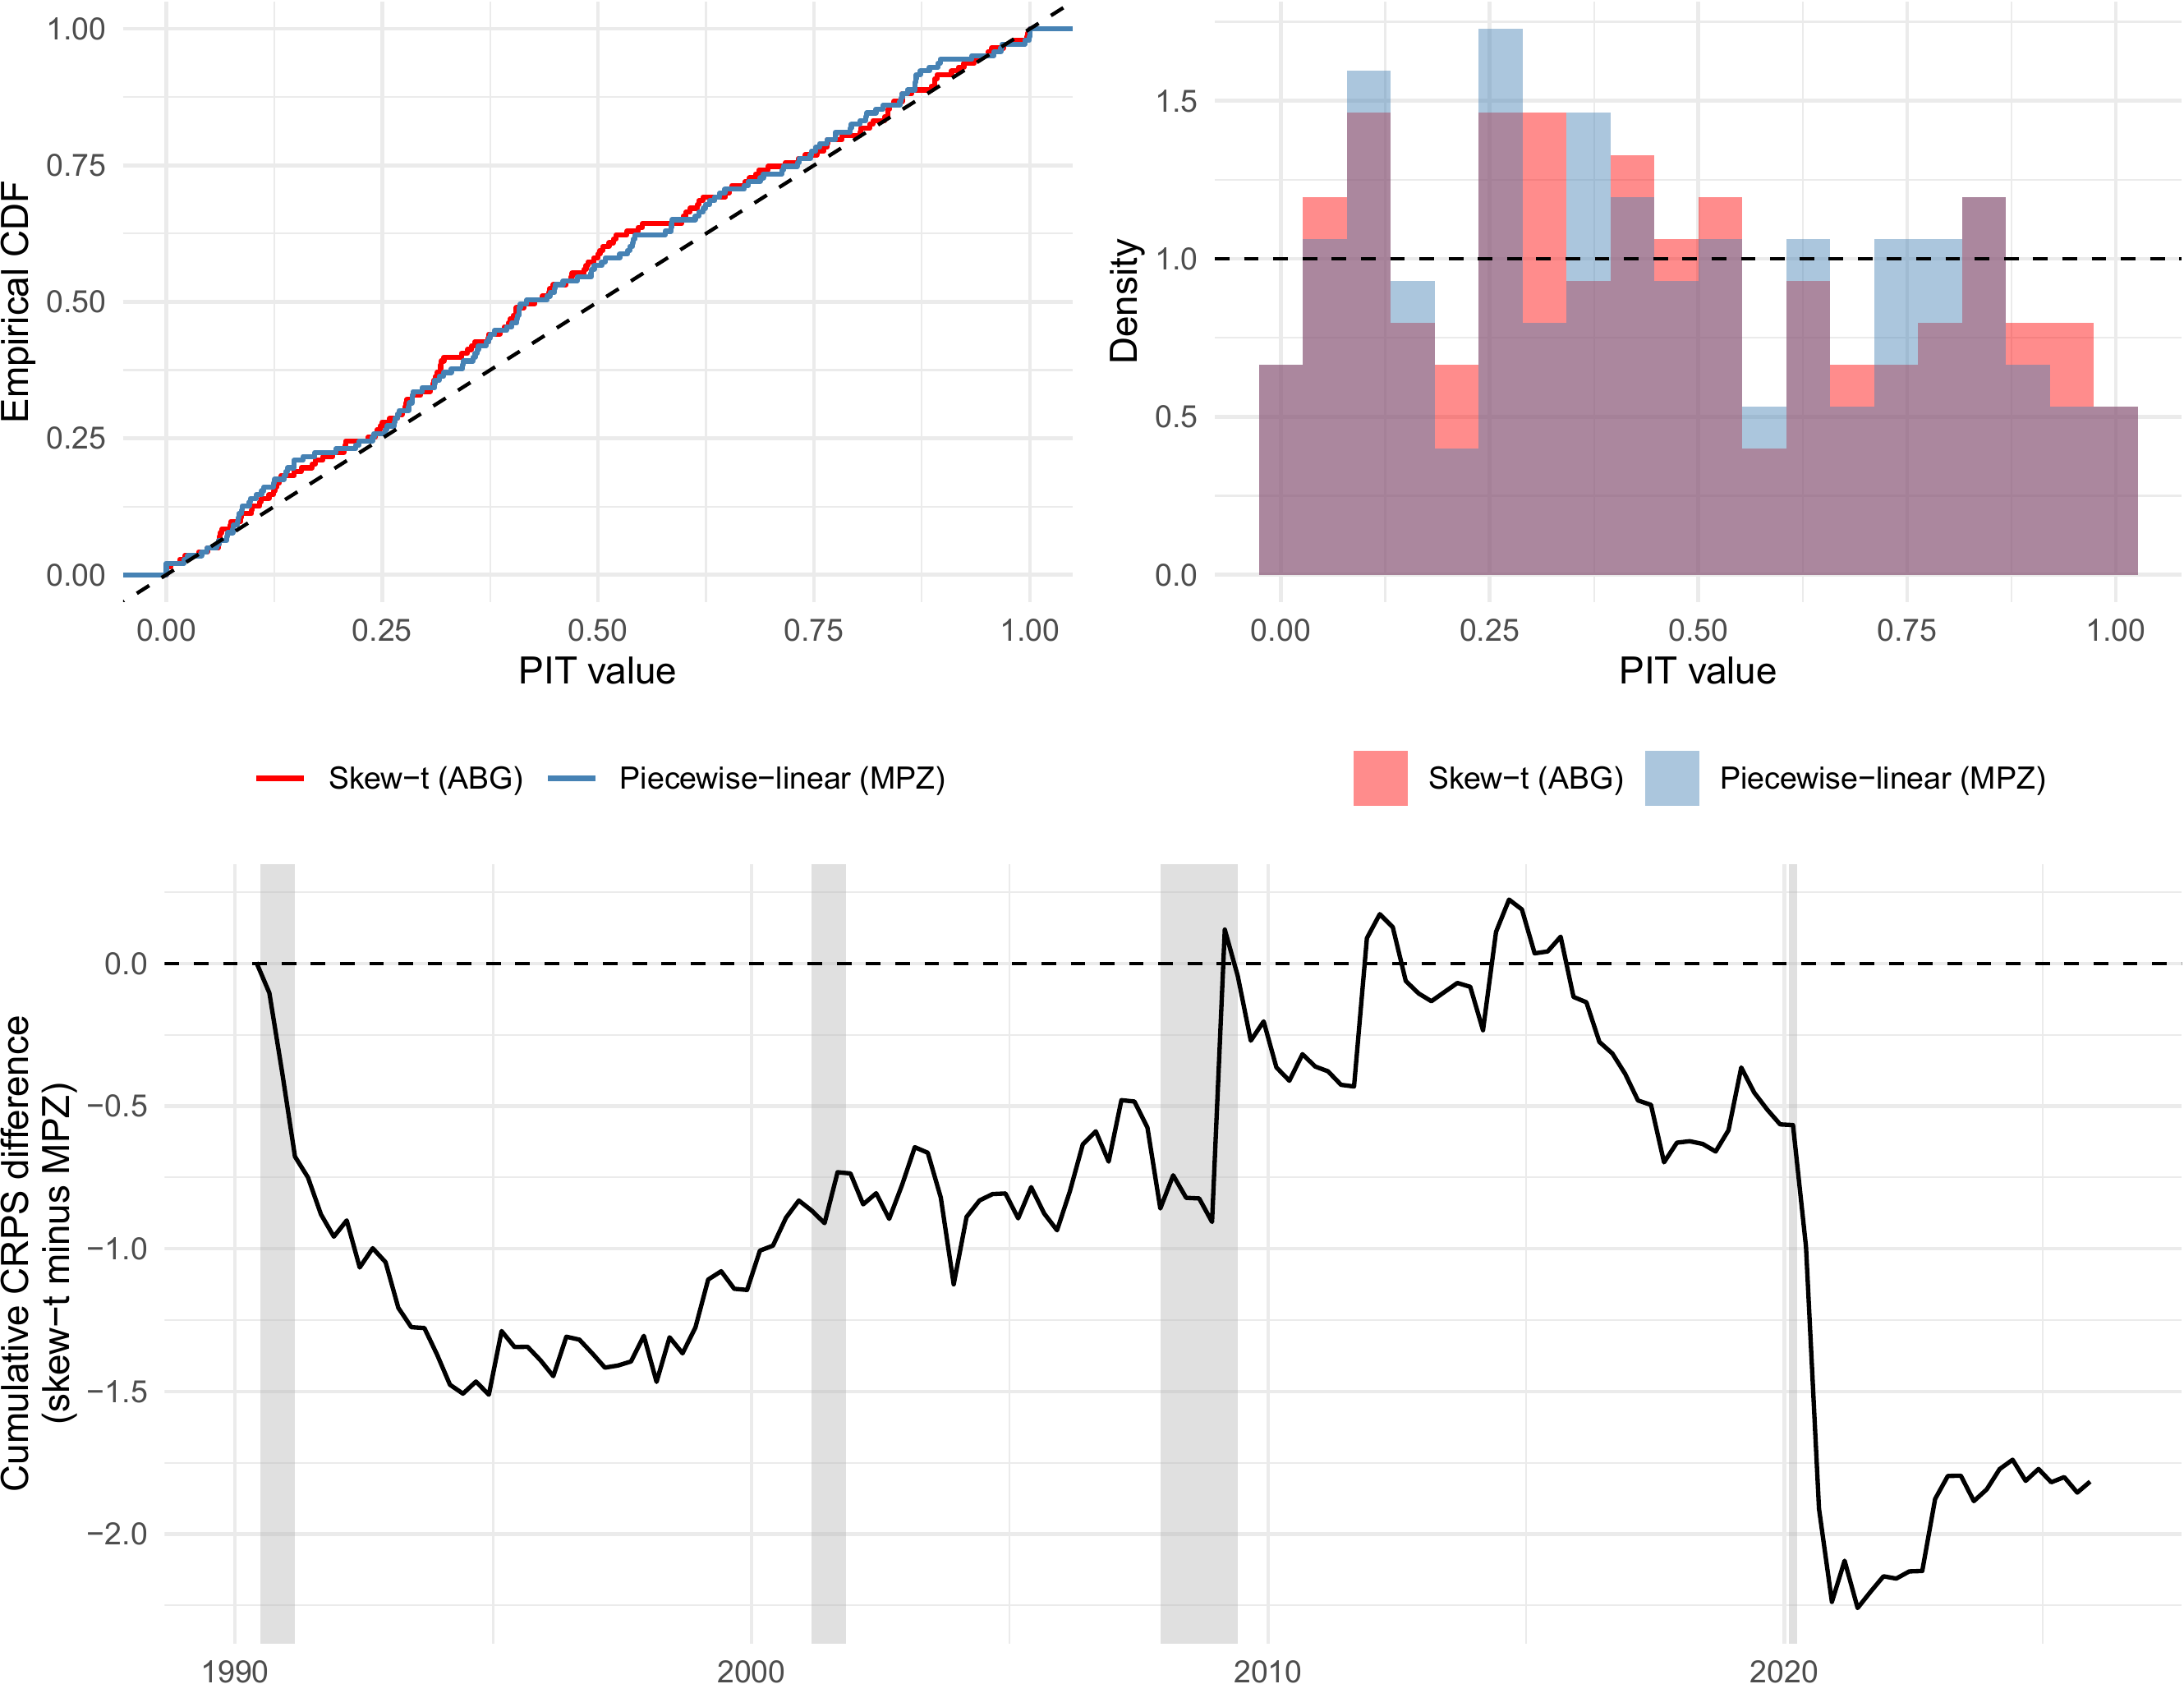
\includegraphics[width=\textwidth]{fig_oos_evaluation.png}}
\end{figure}

\subsection{Design}
\label{subsec:oos-design}

To evaluate out-of-sample predictive accuracy, we implement an expanding window design with the first forecast origin in 1990 Q1. This generates 143 sequential one-step-ahead density forecasts spanning 1990 Q2 through 2025 Q4. At each forecast origin, the entire empirical pipeline is re-estimated using only the historical data available up to that period. Specifically, factor extraction, the quantile regressions at all nineteen quantile levels, and the parameters for both the skew-$t$ and MPZ smoothers are updated recursively at every step.

To keep the 143 recursive estimations computationally feasible, we make two simplifications to the estimation design. First, the panel membership is fixed using the full-sample selection criteria rather than dynamically re-screening the cross-section at each origin. Second, the number of extracted factors is held constant at $r = 5$ across all forecast windows, bypassing recursive rank selection. Fixing the underlying predictor space ensures that observed differences in forecast performance stem directly from the density smoothing methods rather than variations in factor selection over time.

The skew-$t$ fit reaches a parameter bound at 72 of the 143 forecast origins, a rate close to the in-sample frequency reported in Section~\ref{sec:densities}. The boundary problem documented there is therefore not an artifact of full-sample estimation.

\subsection{Calibration}
\label{subsec:calibration}

Both the skew-$t$ and MPZ density forecasts are reasonably well calibrated over the 143-quarter evaluation period. The Kolmogorov-Smirnov (KS) and Cramér-von Mises (CvM) test statistics for both smoothers remain below their corresponding 10\% asymptotic critical values, although the skew-$t$ KS statistic lies just below its 10\% critical value (1.215 versus 1.224), while the MPZ statistic of 1.034 is comfortably below it. The resulting Probability Integral Transform (PIT) values, plotted in the top panels of Figure~\ref{fig:oos}, are close to uniform, although both smoothers place too many outcomes below the forecast median (Section~\ref{subsec:coverage}). An important econometric caveat applies to these baseline calibration metrics. Standard critical values for KS and CvM tests assume that the underlying density parameters are fixed and known. In an expanding window setup, however, the extracted factors, quantile regression coefficients, and smoothing parameters are continuously updated at each origin. As highlighted by \textcite{rossi2019alternative}, recursive parameter estimation introduces sample-dependent variability that alters the asymptotic distributions of PIT-based goodness-of-fit tests.

Because adjusting for recursive estimation error requires non-parametric bootstrap procedures tailored to expanding samples, the reported KS and CvM statistics are best interpreted as indicative benchmarks rather than size-correct hypothesis tests. They show no large departure from uniformity within this setting but are not a formal test.

\subsection{Coverage}
\label{subsec:coverage}

Examining empirical coverage across nominal quantile levels reveals a systematic departure at the center of the forecast distribution. At the 0.50 quantile, empirical coverage rates reach 0.580 for the skew-$t$ and 0.566 for the MPZ procedure. Both smoothers exhibit slight optimism at the median, placing realized GDP growth below the predicted 50th percentile more frequently than the nominal threshold dictates.

Crucially, this bias appears with nearly identical magnitude across both smoothing approaches. Because the two second-step procedures map discrete quantiles into continuous densities in different ways (one fits a four-parameter parametric distribution, the other uses piecewise-linear interpolation), the shared distortion most likely originates in the first stage, in the factor-augmented quantile regressions themselves, where the extracted common factors and linear specification slightly overpredict the central location of the target series across the evaluation sample.

\subsection{CRPS}
\label{subsec:crps}

Table~\ref{tab:oos} reports the out-of-sample scores. A Diebold–Mariano test \parencite{diebold1995comparing} of equal predictive accuracy indicates no statistically significant difference between the two smoothers across any of the four CRPS variants. Overall average CRPS stands at 1.8169 for the skew-$t$ and 1.8296 for the MPZ procedure ($t = -0.89$). Decomposing performance into left-tail, central, and right-tail regions produces similarly negligible differences, with $t$-statistics of $-0.86$, $-0.97$, and $-0.56$ respectively. The bottom panel of Figure~\ref{fig:oos} plots the cumulative CRPS difference over the evaluation window.

Excluding the extreme macroeconomic volatility of the 2020 COVID-19 pandemic leaves this core finding unchanged. Across the remaining 139 quarters, the mean CRPS difference narrows to $-0.001$ ($t = -0.08$). The small advantage the skew-$t$ holds over the full sample is therefore attributable almost entirely to the pandemic quarters.

At individual forecast origins, the skew-$t$ has the lower CRPS in 82 of 143 quarters. A two-sided sign test yields a $p$-value of 0.094, which is not significant at the 5 percent level.

\subsection{Log-score}
\label{subsec:logscore}

Evaluating predictive performance through average log-scores is misleading because of their severe sensitivity to near-zero predictive density. The mean log-score heavily favors the skew-$t$ ($-2.495$ versus $-8.048$), but this difference is driven almost entirely by 5 quarters in which the kernel-smoothed MPZ density assigned essentially zero mass to the realized outcome: 2009 Q2, 2014 Q1, 2020 Q1, 2020 Q2, and 2020 Q3. Three of these quarters correspond to boundary PIT values, while 2009 Q2 and 2020 Q3 lie in the extreme right tail, with PITs above 0.999, where the estimated MPZ density is close to zero. On these observations MPZ incurs extreme log-score penalties, reaching as low as $-690.78$. This is the floor of $\log(10^{-300})$ used in the computation, so the MPZ mean log-score depends on that floor.

One of these dates, 2014 Q1, is not a crisis quarter: realized growth of $-1.38$ percent was unremarkable, yet both smoothers placed it in the extreme left tail. The failure there lies in the estimated quantiles rather than in either smoothing procedure.

Focusing on central tendency, the median log-score difference narrows to 0.0592, with a Wilcoxon signed-rank test favoring the skew-$t$ ($p = 0.0284$).

These findings highlight that while the smoothing procedure alters the fitted density shape, overall out-of-sample accuracy remains nearly indistinguishable. In Section~\ref{sec:mc-results}, MPZ outperformed the skew-$t$ on both metrics only when the true density was bimodal. Section~\ref{sec:densities} showed that the MPZ density is visibly multimodal at several dates in this sample, yet that multimodality does not translate into more accurate one-quarter-ahead forecasts. Two readings are consistent with this. The secondary modes may be estimation noise in the underlying quantile regressions, in which case the added flexibility is capturing sampling variation rather than structure. Alternatively they may be genuine features of the conditional density that simply do not improve accuracy at a one-quarter horizon, where the bulk of the forecast distribution dominates any scoring rule. The evidence here does not distinguish between these two readings.

%----------
%	5. CONCLUSION
%----------

\chapter{Conclusion}
\label{ch:conclusion}

The two-step approach to conditional density estimation introduced by \textcite{adrian2019vulnerable} has become a standard tool in applied macroeconomics and finance. The first step, estimation of conditional quantiles by quantile regression, has received substantial methodological attention, most notably in the extension to factor-augmented conditioning information sets. The second step, in which the estimated quantiles are smoothed into a full conditional density, has received considerably less scrutiny, and is typically implemented using the four-parameter skew-$t$ procedure of ABG, who mention alternatives such as spline interpolation only in a footnote. This thesis examines the second step as the central object of interest, asking whether the choice of smoother changes the estimated conditional density and its forecast accuracy.

The methodological pipeline developed in Chapter~\ref{ch:faqr} combines standard principal-components factor extraction with Koenker–Bassett quantile regression, applied to a grid of nineteen quantile levels, and admits any of a family of alternative smoothing procedures as a modular final step. Chapter~\ref{ch:mc} evaluates two of these procedures, the parametric skew-$t$ of ABG and the semi-parametric piecewise-linear procedure of \textcite{mitchell2024constructing}, in a Monte Carlo experiment based on three data-generating processes: a Gaussian benchmark, a skew-$t$, and a bimodal Gaussian mixture. Chapter~\ref{ch:empirical} applies the same two procedures to US real GDP growth over the period 1959 Q3 to 2025 Q4, with conditioning factors extracted from the FRED-QD panel of 114 macroeconomic series.

The Monte Carlo results show, in a setting in which the true conditional density is known, that the choice of smoother has large consequences when the true density is bimodal. Across one hundred replications the piecewise-linear smoother reduces mean integrated squared error by roughly 38 percent relative to the skew-$t$ and attains a higher mean log-score, with paired $t$-statistics of 29.2 and 9.0 respectively. Under the Gaussian benchmark the ranking reverses and the skew-$t$ is more accurate on MISE; under the skew-$t$ DGP the two metrics disagree, with the parametric procedure favored by the log-score and the semi-parametric by MISE. In MISE terms, the margins in both cases are far smaller than in the bimodal case. Inspection of a representative replication shows the source of the bimodal gap. The true density is collapsed by the skew-$t$ into a single broad unimodal peak centered between the two true component means, while the piecewise-linear smoother recovers both modes and the trough between them.

The empirical application to US GDP growth extends this finding to real data, in a setting in which the true conditional density is unknown but the shape of the estimated density under each smoother can be inspected directly. In 2006 Q2, a period of stable expansion, the two smoothers produce nearly indistinguishable densities and the choice of smoother makes little difference. During periods of economic stress, and most clearly at the acute phase of the 2008 financial crisis, the smoothers diverge substantially: the skew-$t$ remains unimodal by construction, while the piecewise-linear smoother reveals a multimodal structure that is entirely absent from the skew-$t$ density. This empirical divergence is consistent with the Monte Carlo evidence and indicates that the smoothing choice has visible consequences for the estimated conditional density, particularly during periods of economic stress.

The out-of-sample evaluation, reported in Section~\ref{sec:oos}, qualifies this conclusion in an important way. Over 143 quarters of recursively estimated one-quarter-ahead density forecasts, neither smoother is significantly more accurate than the other on any variant of the continuous ranked probability score, and the calibration of both is comparable. The choice of smoother therefore changes the shape of the estimated density substantially without measurably improving predictive accuracy at this horizon. The shape difference is present in the Monte Carlo and in the empirical densities, but in the empirical application the scoring rules do not show a corresponding difference in forecast accuracy.

The results give a two part answer to the question in the introduction. First, the choice of smoother affects the shape of the estimated density. The skew-$t$ is unimodal by construction. In the Monte Carlo study this gives it a higher MISE and a lower log-score than the piecewise-linear smoother when the true density is bimodal. In the US data the two smoothers give similar densities in 2006 Q2 but differ at the other dates shown in Figure~\ref{fig:densities}, most clearly in 2008 Q4. The skew-$t$ fit also reaches a parameter bound at 47 percent of the dates in-sample and 50 percent out-of-sample. Second, the choice of smoother does not lead to a significant difference in one-quarter-ahead forecast accuracy as measured by the CRPS. These conclusions apply to the two smoothers, the three data-generating processes and the one-quarter horizon considered here.


%----------
%	Bibliography
%----------

\clearpage
\addcontentsline{toc}{chapter}{References}

\printbibliography[title={References}]



%----------
%	Appendix
%----------

% If your work includes Appendix, you can uncomment the following lines
%\chapter* {Appendix x}
%\pagenumbering{gobble} % Appendix pages are not numbered



\end{document}
